\documentclass[twoside,a4paper,12pt]{book}

\setcounter{tocdepth}{3}
\setcounter{secnumdepth}{3}

% Package for the code documentation generated by sphinx
\usepackage{sphinx}

% Package for table covering multiple pages
\usepackage{pdflscape} % for 'landscape' environment
\usepackage{longtable}

\usepackage[twoside,a4paper,top=2.5cm, left=2cm]{geometry}
\usepackage[T1]{fontenc}
\usepackage[utf8]{inputenc}
\usepackage{graphicx}
\usepackage{float}
\usepackage{appendix}
\usepackage{fancyhdr}
% package for providing the size of columns on tables
\usepackage{array}
\usepackage{xcolor}
\usepackage{color}
% Package for avoiding the issue with the option hidelinks of the package hyperref
\usepackage[colorlinks=true,
            linkcolor=black,
            urlcolor=blue,
            citecolor=black,
            hyperfootnotes=true]{hyperref}
\usepackage{caption}
\usepackage{eurosym}
\usepackage{multirow}
% Package for providing highlights on code
\usepackage{listings}
\usepackage{enumitem}
\usepackage[acronym]{glossaries}
\usepackage{mathtools}
% Package for version history
\usepackage{vhistory}
\DeclarePairedDelimiter{\ceil}{\lceil}{\rceil}

\newcommand{\ada}[1]{\lstinline[style=ada,
keywordstyle=\mdseries,breaklines,backgroundcolor=\color{white}]&#1&}
\newcommand{\asm}[1]{\lstinline[style=sparc,
keywordstyle=\mdseries,breaklines,backgroundcolor=\color{white}]$#1$}
\newcommand{\prog}[1]{\asm{#1}}

\definecolor{dkgreen}{rgb}{0,0.6,0}
\definecolor{gray}{rgb}{0.8,0.8,0.8}
\definecolor{mauve}{rgb}{0.58,0,0.82}
\definecolor{purple2}{RGB}{153,0,153} % there's actually no standard purple
\definecolor{green2}{RGB}{0,153,0} % a darker green

% Define column type for vertical and horizontal alignment
\newcolumntype{M}[1]{>{\centering\arraybackslash}m{#1}}

% json style
\lstset{
    string=[s]{"}{"},
    stringstyle=\color{blue},
    comment=[l]{:},
    commentstyle=\color{black},
}

\lstdefinestyle{xml}{
       language=xml,
        basicstyle=\ttfamily,
        aboveskip= \bigskipamount,
        belowskip= \bigskipamount,
        abovecaptionskip= \medskipamount,
        belowcaptionskip=\bigskipamount,
        xleftmargin=\parindent,
        columns=flexible,
        numbers=left,
        breaklines=true,
        showstringspaces=false
}


\lstdefinestyle{bash}{
       language=bash,
        basicstyle=\ttfamily,
        aboveskip= \bigskipamount,
        belowskip= \bigskipamount,
        abovecaptionskip= \medskipamount,
        belowcaptionskip=\bigskipamount,
        xleftmargin=\parindent,
        columns=flexible,
        showstringspaces=false,
        breaklines=true,
        showstringspaces=false
}

\lstdefinestyle{python}{%
  language=Python,                   % the language
  basicstyle=\ttfamily,   % size of the fonts for the code
  % Color settings to match IDLE style
  keywordstyle=\color{orange},       % core keywords
  keywordstyle={[2]\color{purple2}}, % built-ins
  stringstyle=\color{green2},
  commentstyle=\color{red},
  upquote=true,                      % requires textcomp,
  numbers=left,
  breaklines=true,
  showstringspaces=false
}

\renewcommand{\_}{%
    \textunderscore\hspace{0pt}%
}

\makeglossaries


\begin{document}

\newacronym{boa}{BOA}{Business Operation Analysis}

\newacronym{eboa}{E-BOA}{Engine for Business Operation Analysis}

\newacronym{rdbms}{RDBMS}{Relational Database Management System}

\newacronym{uuid}{UUID}{Universally unique identifier}

\newacronym{pid}{PID}{Process identifier}

\newacronym{api}{API}{Application Programming Interface}

\newacronym{tle}{TLE}{Two Line Elements}

\newacronym{hktm}{HKTM}{House Keeping Telemetry}

\newacronym{dfep}{DFEP}{Demodulator and Front End Processor}

\newacronym{efep}{EFEP}{EDRS Front End Processor}

\newacronym{s2}{S2}{Sentinel-2}

\newacronym{s2mp}{S2MP}{Sentinel-2 Mission Planning}

\newacronym{eisp}{EISP}{EDRS Instrument Source Packet (applicable also to VGS)}

\newacronym{edrs}{EDRS}{European Data Relay System}

\newacronym{dhus}{DHuS}{Data Hub Software}

\newacronym{fos}{FOS}{Flight Operation Segment}

\newacronym{pdgs}{PDGS}{Payload Data Ground Segment}

\newacronym{dim}{DIM}{Data Ingestion Module}

\newacronym{msi}{MSI}{MultiSpectral Instrument}

\newacronym{vcid}{VCID}{Virtual Channel Identifier}

\newacronym{isp}{ISP}{Instrument Source Packet}

\newacronym{anx}{ANX}{Ascending Node Crossing}

\newacronym{dpc}{DPC}{Data Processing Center}

\newacronym{prip}{PRIP}{Production Interface (delivery) Point}

\input{glossary}

\pagestyle{empty}

\pagenumbering{Alph}
% -*-front.tex-*-
%
% Cover page for the S2BOA documentation
%
% Written by DEIMOS Space S.L. (dibb)
%
% module s2boa

\begin{titlepage}
	
    
\includegraphics[scale=0.20]{deimos_logo.jpg}
    
    \vspace{2.0cm}
    
    	\begin{center}
    
    \vspace{2cm}
    
    \LARGE{\textbf{S2-BOA: Tailoring of BOA for the Sentinel-2 mission}} \\    
    \LARGE{Dynamic data modelling for business operation analysis for Sentinel-2 mission}
    
    	\end{center}    
    
    \vspace{7.0cm}

    \vspace{0.5cm}

    \Large{\textbf{S2-BOA release:} 0.1.0}

    \Large{\textbf{Document release:} 1.0}

    \vspace{1cm}
    
    \large{Date: \today}
    
\end{titlepage}


\cleardoublepage

\setcounter{page}{1}
\pagenumbering{roman}

\frontmatter % Introduction, indexes ...

% Introduction
\begin{versionhistory}
  \vhEntry{1.0}{04.09.2018}{DIBB}{Document created}
  \vhEntry{1.0}{07.09.2018}{DIBB}{Added section for explaining the interface of the component}
  \vhEntry{1.0}{07.09.2018}{DIBB}{Added auto-generated code from the Python docstrings}
  \vhEntry{1.0}{11.09.2018}{DIBB}{Added more explanations for creating an ingestion processor}
  \vhEntry{1.0}{11.09.2018}{DIBB}{Added more explanations for creating an ingestion processor}
  \vhEntry{1.0}{11.09.2018}{DIBB}{Corrected documentation to reflect the new virtual machines created for the testing environment (centos and ubuntu)}
  \vhEntry{1.0}{11.09.2018}{DIBB}{Added section for explaining the generation of this documentation)}
  \vhEntry{1.0}{21.09.2018}{DIBB}{Added explanation for method insert\_and\_erase}

\end{versionhistory}


\tableofcontents
\listoffigures
\listoftables

\mainmatter
\pagestyle{fancy}
\fancyhead{}
\fancyhead[RE]{\slshape \rightmark}
\fancyhead[LO]{\slshape \leftmark}
\fancyfoot{}
\fancyfoot[C]{\lowercase{\thepage}}
\setlength{\headheight}{30pt}

% Introduction
\chapter{Introduction}\label{c:intro}

\acrshort{eboa} is the component aimed to serve as data storage management for business operation analysis. The component aims to allow a dynamic data structure for reducing the effort of developing data models and managing the complex relations between data received.

All the information received is stored into the database using the following high-level entities:

\begin{itemize}

\item Explicit reference: identifier referring to an entity business-related
\item Event: period of time associated to a gauge of a certain aspect business-related
\item Annotation: particular aspect associated to an explicit reference
\item Source: block of information received from the external interface/s to process. After the processing, the interesting information is extracted and stored inside the system.
\item Alert: notification to users regarding anomalies identified by the system related to previous entities.
\item Report: container of analysis.

\end{itemize}


% Purpose and scope
\chapter{Purpose and scope}

The purpose of this document is to explain the tailoring done for \acrshort{s2}\acrshort{boa} component, which is based on \acrshort{boa} for monitoring the mission Sentinel-2. The scope will be limited to explain technically the tailoring.

\acrshort{s2}\acrshort{boa} uses \acrshort{boa}'s infrastructure to store the relevant data received from the external interfaces through the specific ingestion modules and allow its visualization through the specific views.

These are the available specific ingestion modules:

\begin{itemize} 

\item \textbf{ingestion\_nppf}: ingestion module for the planning received from the \acrshort{s2} Mission Planning

\item \textbf{ingestion\_orbpre}: ingestion module for the orbit prediction received from the flight dynamics

\item \textbf{ingestion\_station\_schedule}: ingestion module for the station schedule received from the \acrshort{s2} Mission Planning

\item \textbf{ingestion\_dfep\_schedule}: ingestion module for the \acrshort{dfep} schedule received from the \acrshort{s2} Mission Planning

\item \textbf{ingestion\_slot\_request\_edrs}: ingestion module for the \acrshort{edrs} planning received from the \acrshort{s2} Mission Planning

\item \textbf{ingestion\_station\_acquisition\_report}: ingestion module for the station acquisition report sent by the station operators

\item \textbf{ingestion\_dfep\_acquisition}: ingestion module for the acquisition analysis sent by the station

\item \textbf{ingestion\_edrs\_acquisition}: ingestion module for the \acrshort{edrs} acquisition analysis sent by the \acrshort{eisp}

\item \textbf{ingestion\_vgs\_acquisition}: ingestion module for the station acquisition analysis sent by the \acrshort{eisp}

\item \textbf{ingestion\_dpc}: ingestion module for the processing generation analysis sent by the processor

\item \textbf{ingestion\_ophktm}: ingestion module for inserting the production information of the package, which contains the housekeeping telemetry received from the satellite, generated by \acrshort{pdgs} to be sent to \acrshort{fos}

\item \textbf{ingestion\_rep\_arc}: ingestion module for the indexing of products

\item \textbf{ingestion\_ai}: ingestion module for the archiving of products

\item \textbf{ingestion\_dc}: ingestion module for the circulation of products

\item \textbf{ingestion\_lta}: ingestion module for the long-term-archive of products

\item \textbf{ingestion\_ltas}: ingestion module for the long-term-archive of products

\item \textbf{ingestion\_dam}: ingestion module for the data access management of products

\item \textbf{ingestion\_dhus}: ingestion module for the data availability of products to users

\end{itemize}

These are the available specific views:

\begin{itemize} 

\item \textbf{Planning}: view for planning study

\item \textbf{\acrshort{tle} workflow}: view for the study of \acrshort{tle} circulation towards the expected destinations

\item \textbf{Tracking}: view for following the \acrshort{s2} constellation
  
\item \textbf{Acquisition}: view for acquisition performance from planning study

\item \textbf{\acrshort{hktm} workflow}: view for the study of \acrshort{hktm} circulation towards the expected destinations

\item \textbf{Data availability at \acrshort{dhus}}: view for the study of the dissemination of production towards \acrshort{dhus}

\item \textbf{Sensing data volumes}: view for the study of the volume of data, query driven by sensing timings

\item \textbf{Archive data volumes}: view for the study of the volume of data, query driven by archiving timings
  
\end{itemize}


% Ingestion modules
\chapter{Ingestion modules}

\acrshort{s2}\acrshort{boa} implements ingestion modules for the areas of data shown in figure \ref{fg:data_flow_s2boa}. This data is received inside files (ussually in XML format) from the Sentinel-2 \acrshort{pdgs}, stations and \acrshort{fos}.

\begin{figure}[H]
  \begin{center}
	\centering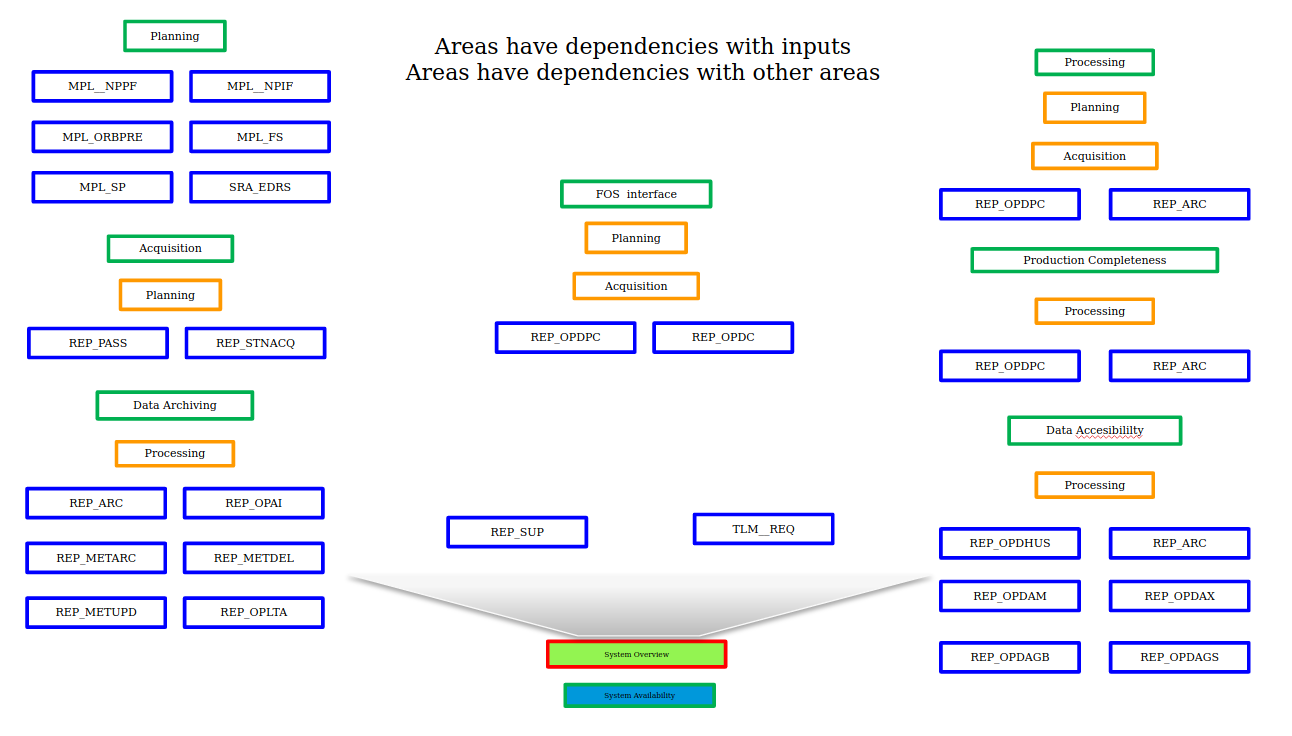
\includegraphics[width=150mm]{../fig/data_flow_s2boa.png}
	\caption{Areas of data related to the S2 mission}
	\label{fg:data_flow_s2boa}
  \end{center}
\end{figure}


This chapter describes each of the ingestion modules in the following sections. The figure \ref{fg:legened_structure_of_ingestions} shows the legend for the diagrams, used to represent the data stored.

\begin{figure}[H]
  \begin{center}
	\centering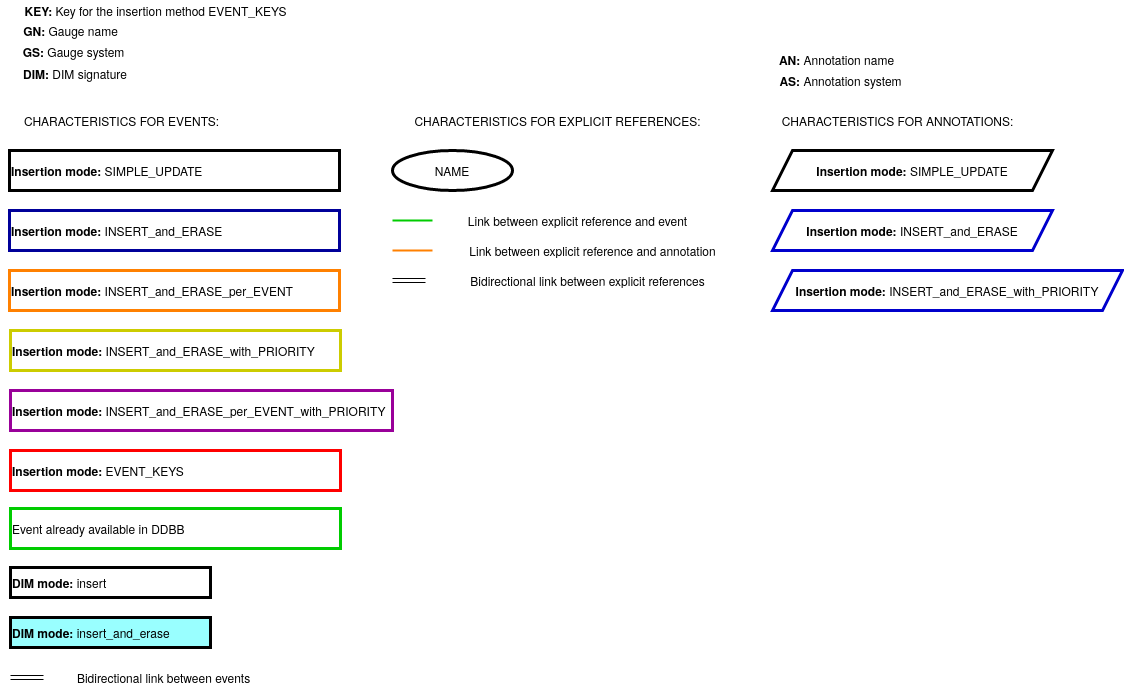
\includegraphics[width=75mm]{../fig/legened_structure_of_ingestions.png}
	\caption{Legend for the diagrams, used to represent the data stored}
	\label{fg:legened_structure_of_ingestions}
  \end{center}
\end{figure}

% Ingestion NPPF
\section{Ingestion module for the MPL\_NPPF file}

This sections describes the ingestion module for inserting the planning of operations commanding the satellite.

The associated ingestion processor is:

\begin{itemize} 

\item \textbf{s2boa.ingestions.ingestion\_nppf.ingestion\_nppf}
  
\end{itemize}

This module uses the following \acrshort{dim} signatures:

\begin{itemize} 

\item \textbf{NPPF\_XXX}: data corresponding to the planning of operations commanding the satellite.

\item \textbf{CORRECTED\_NPPF\_XXX}: data corresponding to the planning of operations commanding the satellite corrected by the available orbit prediction data.

\item \textbf{COMPLETENESS\_NPPF\_XXX}: data corresponding to the definition of planning completeness used for analysis.
  
\end{itemize}

Where XXX is the corresponding satellite id.

The figure \ref{fg:structure_ingestion_nppf} shows a simplified diagram of the structure of events inserted (associated structure of values not included for simplicity).

\begin{figure}[H]
  \begin{center}
	\centering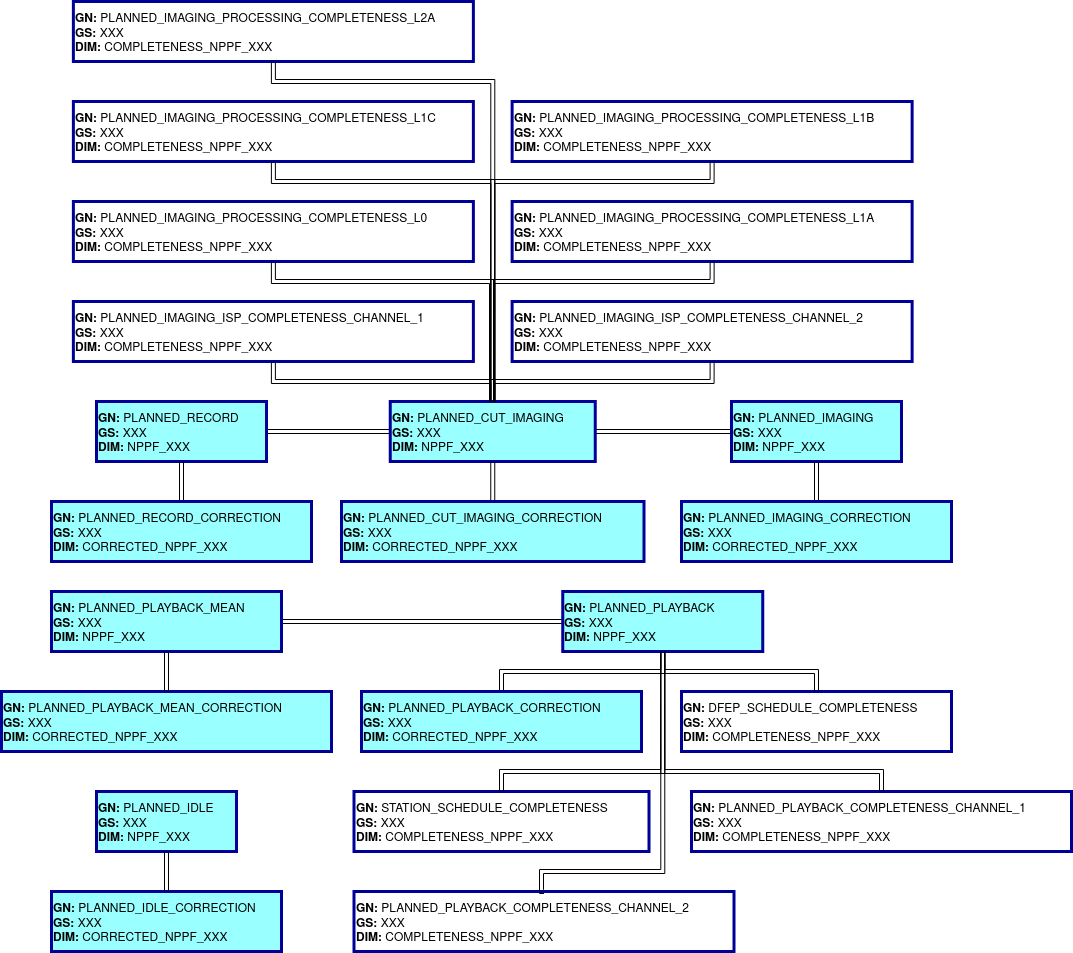
\includegraphics[width=150mm]{../fig/structure_ingestion_nppf.png}
	\caption{Structure of events inserted by the ingestion module for the MPL\_NPPF file}
	\label{fg:structure_ingestion_nppf}
  \end{center}
\end{figure}

The table \ref{tb:description_events_ingestion_nppf} shows the description of the events inserted by the ingestion.

\begin{landscape}
\begin{longtable}{|M{0.15\linewidth}|M{0.05\linewidth}|M{0.10\linewidth}|M{0.10\linewidth}|M{0.15\linewidth}|M{0.15\linewidth}|M{0.15\linewidth}|}
\hline \textbf{Gauge name} & \textbf{Gauge system} & \textbf{DIM signature} & \textbf{Insertion mode} & \textbf{Description} & \textbf{Start} & \textbf{Stop} \\ \hline
\textbf{PLANNED\_RECORD} & XXX & NPPF\_XXX & INSERT\_and\_ERASE (insert\_and\_erase) & Event for representing the \textbf{recording operation} & UTC time associated to command 'MPMMRNOM' or 'MPMMRNRT' & UTC time associated to command 'MPMMRSTP' or 'MPMMRNRT' or 'MPMMRNOM' \\ \hline
\textbf{PLANNED\_CUT\_IMAGING} & XXX & NPPF\_XXX & INSERT\_and\_ERASE (insert\_and\_erase) & Event for representing the \textbf{imaging operation associated to a specific recording operation} & UTC time associated to command 'MPMSSCAL' or 'MPMSDASC' or 'MPMSDCLO' or 'MPMSIVIC' or 'MPMSNOBS' or 'MPMSIRAW' or 'MPMSIDTS' or 'MPMMRNOM' or 'MPMMRNRT' & UTC time associated to command 'MPMSIMID' or 'MPMSIDSB' or 'MPMMRSTP' or 'MPMMRNRT' or 'MPMMRNOM' \\ \hline
\textbf{PLANNED\_IMAGING} & XXX & NPPF\_XXX & INSERT\_and\_ERASE (insert\_and\_erase) & Event for representing the \textbf{imaging operation} covering one or several planned recording operations & UTC time associated to command 'MPMSSCAL' or 'MPMSDASC' or 'MPMSDCLO' or 'MPMSIVIC' or 'MPMSNOBS' or 'MPMSIRAW' or 'MPMSIDTS' & UTC time associated to command 'MPMSIMID' or 'MPMSIDSB' or 'MPMMRSTP' \\ \hline
\textbf{PLANNED\_PLAYBACK} & XXX & NPPF\_XXX & INSERT\_and\_ERASE (insert\_and\_erase) & Event for representing the \textbf{playback operation} & UTC time associated to command 'MPMMPNOM' or 'MPMMPREG' or 'MPMMPBRT' or 'MPMMPNRT' & UTC time associated to command 'MPMMPSTP' \\ \hline
\textbf{PLANNED\_PLAYBACK\_MEAN} & XXX & NPPF\_XXX & INSERT\_and\_ERASE (insert\_and\_erase) & Event for representing the \textbf{mean of the playback operation} & UTC time associated to command 'MPXBSBOP' or 'MPG1STRT' or 'MPG2STRT' & UTC time associated to command 'MPXBOPSB' (when start is associated to command 'MPXBSBOP') or 'MPOCPRY2' (when start is associated to command 'MPG1STRT' or 'MPG2STRT') \\ \hline
\textbf{PLANNED\_IDLE} & XXX & NPPF\_XXX & INSERT\_and\_ERASE (insert\_and\_erase) & Event for representing the \textbf{idle state} & UTC time associated to command 'MPMSIMID' or 'MPMSSBID' & UTC time associated to command 'MPMSSCAL' or 'MPMSDASC' or 'MPMSDCLO' or 'MPMSIVIC' or 'MPMSNOBS' or 'MPMSIRAW' or 'MPMSIDTS' or 'MPMSIDSB' \\ \hline
\textbf{***\_CORRECTION} & XXX & \- CORRECTED\_NPPF\_XXX & INSERT\_and\_ERASE (insert\_and\_erase) & Event for representing the \textbf{planning events corrected using the orbit prediction events} & Start of the planned event corrected using the ORBPRE & Stop of the planned event corrected using the ORBPRE \\ \hline
\textbf{DFEP\_SCHEDULE\_COMPLETENESS} & XXX & \- COMPLETENESS & INSERT\_and\_ERASE (insert) & Event for representing the \textbf{expectation of the DFEP schedule} & Corrected start of the planned playback + 2s (SAD/HKTM) or + 9s (MSI); (if start \textgreater  stop) Corrected stop of the planned playback - 4s & Start (SAD/HKTM) or Corrected stop of the planned playback - 9s (MSI); (if start \textgreater  stop) Corrected stop of the planned playback - 3s \\ \hline
\textbf{STATION\_SCHEDULE\_COMPLETENESS} & XXX & \- COMPLETENESS\_NPPF\_XXX & INSERT\_and\_ERASE (insert) & Event for representing the \textbf{expectation of the Station schedule} & Corrected start of the planned playback + 2s (SAD/HKTM) or + 9s (MSI); (if start \textgreater  stop) Corrected stop of the planned playback - 4s & Start (SAD/HKTM) or Corrected stop of the planned playback - 9s (MSI); (if start \textgreater  stop) Corrected stop of the planned playback - 3s \\ \hline
\textbf{PLANNED\_PLAYBACK\_COMPLETENESS\_CHANNEL\_1} & XXX & \- COMPLETENESS\_NPPF\_XXX & INSERT\_and\_ERASE (insert) & Event for representing the \textbf{expectation of the planned playbacks using the channel 1} & Corrected start of the planned playback + 2s (SAD/HKTM) or + 9s (MSI); (if start \textgreater  stop) Corrected stop of the planned playback - 4s & Start (SAD/HKTM) or Corrected stop of the planned playback - 9s (MSI); (if start \textgreater  stop) Corrected stop of the planned playback - 3s \\ \hline
\textbf{PLANNED\_PLAYBACK\_COMPLETENESS\_CHANNEL\_2} & XXX & \- COMPLETENESS\_NPPF\_XXX & INSERT\_and\_ERASE (insert) & Event for representing the \textbf{expectation of the planned playbacks using the channel 2} & Corrected start of the planned playback + 2s (SAD/HKTM) or + 9s (MSI); (if start \textgreater  stop) Corrected stop of the planned playback - 4s & Start (SAD/HKTM) or Corrected stop of the planned playback - 9s (MSI); (if start \textgreater  stop) Corrected stop of the planned playback - 3s \\ \hline
\textbf{PLANNED\_IMAGING\_ISP\_COMPLETENESS\_CHANNEL\_1} & XXX & \- COMPLETENESS\_NPPF\_XXX & INSERT\_and\_ERASE (insert) & Event for representing the \textbf{expectation of the planned imaging using the channel 1} & Corrected start of the planned imaging + 10s; (if start \textgreater  stop) Corrected stop of the planned imaging - 12s & Corrected stop of the planned imaging - 10s; (if start \textgreater  stop) Corrected stop of the planned imaging - 6s \\ \hline
\textbf{PLANNED\_IMAGING\_ISP\_COMPLETENESS\_CHANNEL\_2} & XXX & \- COMPLETENESS\_NPPF\_XXX & INSERT\_and\_ERASE (insert) & Event for representing the \textbf{expectation of the planned imaging using the channel 2} & Corrected start of the planned imaging + 10s; (if start \textgreater  stop) Corrected stop of the planned imaging - 12s & Corrected stop of the planned imaging - 10s; (if start \textgreater  stop) Corrected stop of the planned imaging - 6s \\ \hline
\textbf{PLANNED\_IMAGING\_PROCESSING\_COMPLETENESS\_L0} & XXX & \- COMPLETENESS\_NPPF\_XXX & INSERT\_and\_ERASE (insert) & Event for representing the \textbf{expectation of the processing of the planned imaging for the L0} & Corrected start of the planned imaging + 10s; (if start \textgreater  stop) Corrected stop of the planned imaging - 12s & Corrected stop of the planned imaging - 10s; (if start \textgreater  stop) Corrected stop of the planned imaging - 6s \\ \hline
\textbf{PLANNED\_IMAGING\_PROCESSING\_COMPLETENESS\_L1A} & XXX & \- COMPLETENESS\_NPPF\_XXX & INSERT\_and\_ERASE (insert) & Event for representing the \textbf{expectation of the processing of the planned imaging for the L1A} & Corrected start of the planned imaging + 10s; (if start \textgreater  stop) Corrected stop of the planned imaging - 12s & Corrected stop of the planned imaging - 10s; (if start \textgreater  stop) Corrected stop of the planned imaging - 6s \\ \hline
\textbf{PLANNED\_IMAGING\_PROCESSING\_COMPLETENESS\_L1B} & XXX & \- COMPLETENESS\_NPPF\_XXX & INSERT\_and\_ERASE (insert) & Event for representing the \textbf{expectation of the processing of the planned imaging for the L1B} & Corrected start of the planned imaging + 10s; (if start \textgreater  stop) Corrected stop of the planned imaging - 12s & Corrected stop of the planned imaging - 10s; (if start \textgreater  stop) Corrected stop of the planned imaging - 6s \\ \hline
\textbf{PLANNED\_IMAGING\_PROCESSING\_COMPLETENESS\_L1C} & XXX & \- COMPLETENESS\_NPPF\_XXX & INSERT\_and\_ERASE (insert) & Event for representing the \textbf{expectation of the processing of the planned imaging for the L1C} & Corrected start of the planned imaging + 10s; (if start \textgreater  stop) Corrected stop of the planned imaging - 12s & Corrected stop of the planned imaging - 10s; (if start \textgreater  stop) Corrected stop of the planned imaging - 6s \\ \hline
\textbf{PLANNED\_IMAGING\_PROCESSING\_COMPLETENESS\_L2A} & XXX & \- COMPLETENESS\_NPPF\_XXX & INSERT\_and\_ERASE (insert) & Event for representing the \textbf{expectation of the processing of the planned imaging for the L2A} & Corrected start of the planned imaging + 10s; (if start \textgreater  stop) Corrected stop of the planned imaging - 12s & Corrected stop of the planned imaging - 10s; (if start \textgreater  stop) Corrected stop of the planned imaging - 6s \\ \hline
\caption{Table describing the events associated to the ingestion}
\label{tb:description_events_ingestion_nppf}
\end{longtable}
\end{landscape}

\subsection{Ingestion details}

This section describes some ingestion details for inserting the data. In particular:

\begin{itemize} 

\item The correction of the generation time when is greater than the validity start
  
\end{itemize}

\subsubsection{Correction of the generation time}

Due to an operation procedure using the \acrshort{s2mp}, the generation time could be greater than the validity start. This could result into having deprecated data in the DDBB.

To solve this issue the processor changes the generation time to be the validity start when the first is greater.


% Ingestion ORBPRE
\section{Ingestion module for the MPL\_ORBPRE file}

This sections describes the ingestion module for inserting the orbit prediction of the satellites generated by \acrshort{fos}.

The associated ingestion processor is:

\begin{itemize} 

\item \textbf{s2boa.ingestions.ingestion\_orbpre.ingestion\_orbpre}
  
\end{itemize}

This module uses the following \acrshort{dim} signatures:

\begin{itemize} 

\item \textbf{ORBPRE}: data corresponding to the orbit prediction of the satellites generated by \acrshort{fos} used for adjusting the timing of the planning events which are using the operations angle.

\item \textbf{CORRECTED\_NPPF\_XXX}: data corresponding to the planning of operations commanding the satellite corrected by the available orbit prediction data.

\item \textbf{COMPLETENESS\_NPPF\_XXX}: data corresponding to the definition of planning completeness used for analysis. \textbf{Priority is equal to 20}.
  
\end{itemize}

Where XXX is the corresponding satellite id.

The figure \ref{fg:structure_ingestion_orbpre} shows a simplified diagram of the structure of events inserted (associated structure of values not included for simplicity).

\begin{figure}[H]
  \begin{center}
	\centering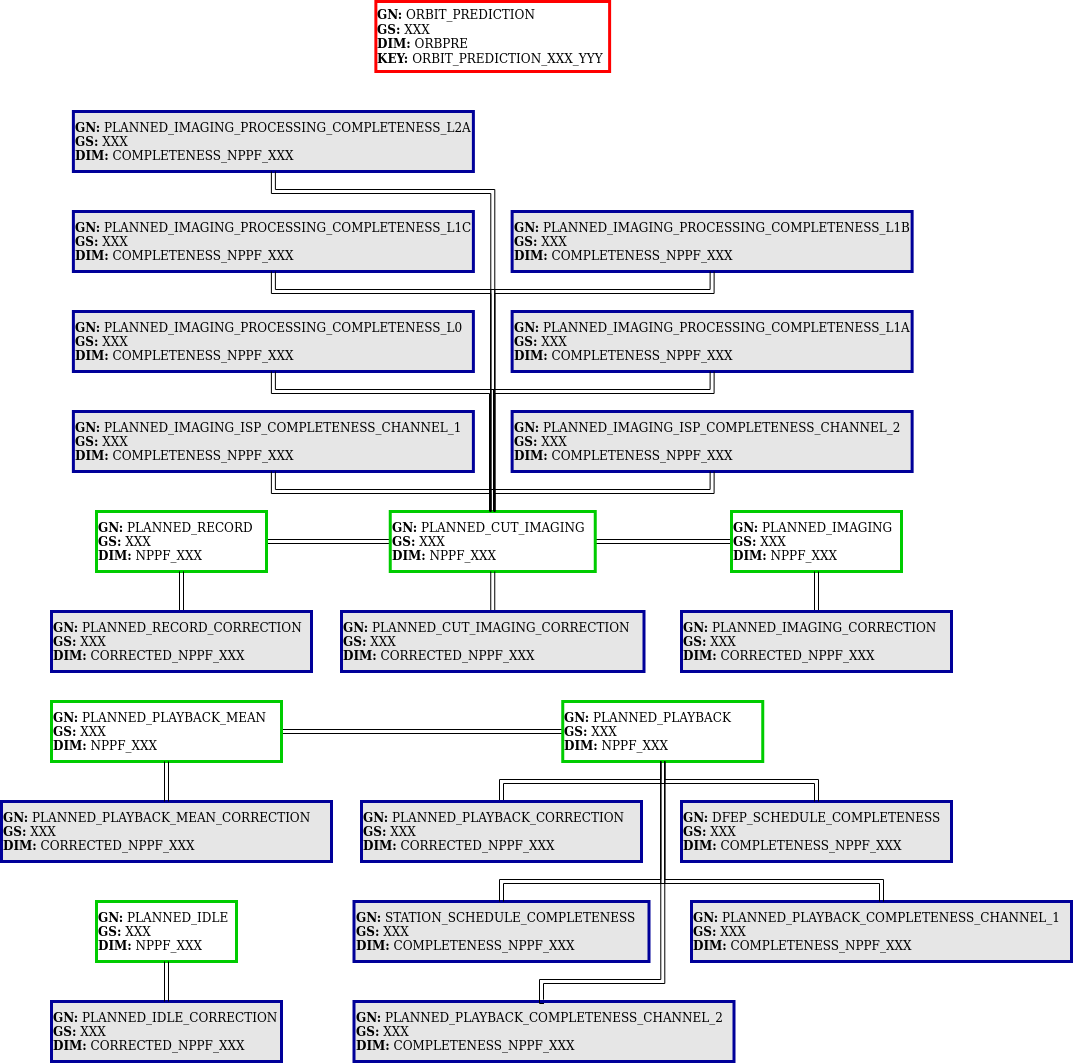
\includegraphics[width=150mm]{../fig/structure_ingestion_orbpre.png}
	\caption{Structure of events inserted by the ingestion module for the MPL\_ORBPRE file}
	\label{fg:structure_ingestion_orbpre}
  \end{center}
\end{figure}

Where YYY is the orbit number.

The table \ref{tb:description_events_ingestion_orbpre} shows the description of the events inserted by the ingestion.

\begin{landscape}
\begin{longtable}{|M{0.15\linewidth}|M{0.05\linewidth}|M{0.10\linewidth}|M{0.10\linewidth}|M{0.15\linewidth}|M{0.15\linewidth}|M{0.15\linewidth}|}
\hline \textbf{Gauge name} & \textbf{Gauge system} & \textbf{DIM signature} & \textbf{Insertion mode} & \textbf{Description} & \textbf{Start} & \textbf{Stop} \\ \hline
\textbf{ORBIT\_PREDICTION} & XXX & ORBIT\_PREDICTION\_XXX\_YYY & EVENT\_KEYS (insert) [KEY: ORBIT\_PREDICTION\_XXX\_YYY] & Event for representing the \textbf{orbit predition information of a specific orbit} & UTC time related to the ANX of orbit N & UTC time related to the ANX of orbit N + 1 \\ \hline
\textbf{***\_CORRECTION} & XXX & \- CORRECTED\_NPPF\_XXX & INSERT\_and\_ERASE (insert\_and\_erase) & Event for representing the \textbf{planning events corrected using the orbit prediction events} & Start of the planned event corrected using the ORBPRE & Stop of the planned event corrected using the ORBPRE \\ \hline
\textbf{DFEP\_SCHEDULE\_COMPLETENESS} & XXX & \- COMPLETENESS\_NPPF\_XXX & INSERT\_and\_ERASE\_with\_PRIORITY (insert) & Event for representing the \textbf{expectation of the DFEP schedule} & Corrected start of the planned playback + 2s (SAD/HKTM) or + 9s (MSI); (if start \textgreater  stop) Corrected stop of the planned playback - 4s & Start (SAD/HKTM) or Corrected stop of the planned playback - 9s (MSI); (if start \textgreater  stop) Corrected stop of the planned playback - 3s \\ \hline
\textbf{STATION\_SCHEDULE\_COMPLETENESS} & XXX & \- COMPLETENESS\_NPPF\_XXX & INSERT\_and\_ERASE\_with\_PRIORITY (insert) & Event for representing the \textbf{expectation of the Station schedule} & Corrected start of the planned playback + 2s (SAD/HKTM) or + 9s (MSI); (if start \textgreater  stop) Corrected stop of the planned playback - 4s & Start (SAD/HKTM) or Corrected stop of the planned playback - 9s (MSI); (if start \textgreater  stop) Corrected stop of the planned playback - 3s \\ \hline
\textbf{PLANNED\_PLAYBACK\_COMPLETENESS\_CHANNEL\_1} & XXX & \- COMPLETENESS\_NPPF\_XXX & INSERT\_and\_ERASE\_with\_PRIORITY (insert) & Event for representing the \textbf{expectation of the planned playbacks using the channel 1} & Corrected start of the planned playback + 2s (SAD/HKTM) or + 9s (MSI); (if start \textgreater  stop) Corrected stop of the planned playback - 4s & Start (SAD/HKTM) or Corrected stop of the planned playback - 9s (MSI); (if start \textgreater  stop) Corrected stop of the planned playback - 3s \\ \hline
\textbf{PLANNED\_PLAYBACK\_COMPLETENESS\_CHANNEL\_2} & XXX & \- COMPLETENESS\_NPPF\_XXX & INSERT\_and\_ERASE\_with\_PRIORITY (insert) & Event for representing the \textbf{expectation of the planned playbacks using the channel 2} & Corrected start of the planned playback + 2s (SAD/HKTM) or + 9s (MSI); (if start \textgreater  stop) Corrected stop of the planned playback - 4s & Start (SAD/HKTM) or Corrected stop of the planned playback - 9s (MSI); (if start \textgreater  stop) Corrected stop of the planned playback - 3s \\ \hline
\textbf{PLANNED\_IMAGING\_ISP\_COMPLETENESS\_CHANNEL\_1} & XXX & \- COMPLETENESS\_NPPF\_XXX & INSERT\_and\_ERASE\_with\_PRIORITY (insert) & Event for representing the \textbf{expectation of the planned imaging using the channel 1} & Corrected start of the planned imaging + 10s; (if start \textgreater  stop) Corrected stop of the planned imaging - 12s & Corrected stop of the planned imaging - 10s; (if start \textgreater  stop) Corrected stop of the planned imaging - 6s \\ \hline
\textbf{PLANNED\_IMAGING\_ISP\_COMPLETENESS\_CHANNEL\_2} & XXX & \- COMPLETENESS\_NPPF\_XXX & INSERT\_and\_ERASE\_with\_PRIORITY (insert) & Event for representing the \textbf{expectation of the planned imaging using the channel 2} & Corrected start of the planned imaging + 10s; (if start \textgreater  stop) Corrected stop of the planned imaging - 12s & Corrected stop of the planned imaging - 10s; (if start \textgreater  stop) Corrected stop of the planned imaging - 6s \\ \hline
\textbf{PLANNED\_IMAGING\_PROCESSING\_COMPLETENESS\_L0} & XXX & \- COMPLETENESS\_NPPF\_XXX & INSERT\_and\_ERASE\_with\_PRIORITY (insert) & Event for representing the \textbf{expectation of the processing of the planned imaging for the L0} & Corrected start of the planned imaging + 10s; (if start \textgreater  stop) Corrected stop of the planned imaging - 12s & Corrected stop of the planned imaging - 10s; (if start \textgreater  stop) Corrected stop of the planned imaging - 6s \\ \hline
\textbf{PLANNED\_IMAGING\_PROCESSING\_COMPLETENESS\_L1A} & XXX & \- COMPLETENESS\_NPPF\_XXX & INSERT\_and\_ERASE\_with\_PRIORITY (insert) & Event for representing the \textbf{expectation of the processing of the planned imaging for the L1A} & Corrected start of the planned imaging + 10s; (if start \textgreater  stop) Corrected stop of the planned imaging - 12s & Corrected stop of the planned imaging - 10s; (if start \textgreater  stop) Corrected stop of the planned imaging - 6s \\ \hline
\textbf{PLANNED\_IMAGING\_PROCESSING\_COMPLETENESS\_L1B} & XXX & \- COMPLETENESS\_NPPF\_XXX & INSERT\_and\_ERASE\_with\_PRIORITY (insert) & Event for representing the \textbf{expectation of the processing of the planned imaging for the L1B} & Corrected start of the planned imaging + 10s; (if start \textgreater  stop) Corrected stop of the planned imaging - 12s & Corrected stop of the planned imaging - 10s; (if start \textgreater  stop) Corrected stop of the planned imaging - 6s \\ \hline
\textbf{PLANNED\_IMAGING\_PROCESSING\_COMPLETENESS\_L1C} & XXX & \- COMPLETENESS\_NPPF\_XXX & INSERT\_and\_ERASE\_with\_PRIORITY (insert) & Event for representing the \textbf{expectation of the processing of the planned imaging for the L1C} & Corrected start of the planned imaging + 10s; (if start \textgreater  stop) Corrected stop of the planned imaging - 12s & Corrected stop of the planned imaging - 10s; (if start \textgreater  stop) Corrected stop of the planned imaging - 6s \\ \hline
\textbf{PLANNED\_IMAGING\_PROCESSING\_COMPLETENESS\_L2A} & XXX & \- COMPLETENESS\_NPPF\_XXX & INSERT\_and\_ERASE\_with\_PRIORITY (insert) & Event for representing the \textbf{expectation of the processing of the planned imaging for the L2A} & Corrected start of the planned imaging + 10s; (if start \textgreater  stop) Corrected stop of the planned imaging - 12s & Corrected stop of the planned imaging - 10s; (if start \textgreater  stop) Corrected stop of the planned imaging - 6s \\ \hline
\caption{Table describing the events associated to the ingestion}
\label{tb:description_events_ingestion_orbpre}
\end{longtable}
\end{landscape}

\subsection{Ingestion details}

This section describes some ingestion details for inserting the data. In particular:

\begin{itemize} 

\item The algorithm to correct the timing of the planning events

\item The correction of the generation time to avoid overriding data used for completeness analysis
  
\end{itemize}

\subsubsection{Algorithm to correct the timing of the planning events}

The algorithm to correct the timing of the planning events is as follows:

For every planning event:

\begin{itemize} 

\item Get satellite ID, start and stop orbits and start and stop angles.

\item Get the \acrshort{anx} time from the orbit prediction information covering the previous orbits and the following ones

\item Apply the following formula to the start and stop angles (\(\alpha\)) using the orbital period (p) and the corresponding \acrshort{anx} timing (t):

  \(sin_1 = sin(\alpha)\)

  \(sin_2 = sin(2*\alpha)\)

  \(cos_1 = cos(\alpha)\)

  \(cos_2 = cos(2*\alpha)\)

  \(cos_3 = cos(3*\alpha)\)

  Adjust angle to a circunference (perfect distribution in 360º):
  
  \(m = \alpha - 0.13175612 - 2*(-0.0001529)*sin_1 - 2*(-0.0660818)*cos_1 - 2*0.16855853*sin_2 - 2*(-0.0007759)*cos_2 - 2*0.0009872*cos_3 - 2*0.00687159*sin_2\)

  Transform angle to \(\delta\) time:
  
  \(s = (m * p)/360.0\)

  \(UTC time = t + s \)
  
\end{itemize}

\subsubsection{Correction of the generation time}

The validity start of the ORBPRE is almost equal to the generation time. This makes the data extracted to be in priority with respect to the data extracted of other components which would need to be in priority.

To solve this issue the processor changes the generation time to be the generation time minus 1 day.


% Ingestion MPL_SP
\section{Ingestion module for the MPL\_SP file}

This sections describes the ingestion module for inserting the station schedule information received from the S2 Mission Planning.

The associated ingestion processors are:

\begin{itemize} 

\item \textbf{s2boa.ingestions.ingestion\_station\_schedule.ingestion\_station\_schedule}
  
\end{itemize}

This module uses the following \acrshort{dim} signatures:

\begin{itemize} 

\item \textbf{STATION\_SCHEDULE\_WWW\_XXX}: data corresponding to station schedule information associated to a specific station and satellite received from the Mission Planning.

\item \textbf{COMPLETENESS\_NPPF\_XXX}: data corresponding to the definition of planning completeness used for analysis.
  
\end{itemize}

Where XXX is the corresponding satellite id and WWW to the station ID.

The figure \ref{fg:structure_ingestion_station_schedule} shows a simplified diagram of the structure of events inserted (associated structure of values not included for simplicity).

\begin{figure}[H]
  \begin{center}
	\centering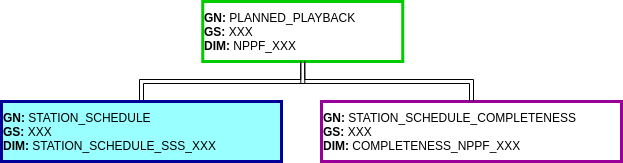
\includegraphics[width=150mm]{structure_ingestion_station_schedule.png}
	\caption{Structure of events inserted by the ingestion module for the MPL\_SP file}
	\label{fg:structure_ingestion_station_schedule}
  \end{center}
\end{figure}

The table \ref{tb:description_events_ingestion_station_schedule} shows the description of the events inserted by the ingestion.

\begin{landscape}
\begin{longtable}{|M{0.15\linewidth}|M{0.05\linewidth}|M{0.10\linewidth}|M{0.10\linewidth}|M{0.15\linewidth}|M{0.15\linewidth}|M{0.15\linewidth}|}
\hline \textbf{Gauge name} & \textbf{Gauge system} & \textbf{DIM signature} & \textbf{Insertion mode} & \textbf{Description} & \textbf{Start} & \textbf{Stop} \\ \hline
\textbf{STATION\_SCHEDULE} & XXX & STATION\_SCHEDULE\_WWW\_XXX & ERASE\_and\_REPLACE\_per\_EVENT (insert) & Event for representing the \textbf{station schedule} & UTC value inside the Data\_start node & UTC value inside the Data\_stop node  \\ \hline
\textbf{STATION\_SCHEDULE\_COMPLETENESS} & XXX & \- COMPLETENESS\_NPPF\_XXX & ERASE\_and\_REPLACE (insert\_and\_erase) & Event for representing the \textbf{expectation of the Station schedule} & UTC value inside the Data\_start node & UTC value inside the Data\_stop node  \\ \hline
\caption{Table describing the events associated to the ingestion}
\label{tb:description_events_ingestion_station_schedule}
\end{longtable}
\end{landscape}

\subsection{Ingestion details}

This section describes some ingestion details for inserting the data. In particular:

\begin{itemize} 

\item The correction of the generation time to avoid overriding data used for completeness analysis
  
\end{itemize}

\subsubsection{Correction of the generation time}

The generation time of the data extracted is one day before the validity start. This could be a problem as the processor of the ORBPRE files could override this data.

To solve this issue the processor changes the generation time to be the validity start.


% Ingestion MPL_FS
\section{Ingestion module for the MPL\_FS file}

This sections describes the ingestion module for inserting the DFEP schedule information received from the S2 Mission Planning.

The associated ingestion processor is:

\begin{itemize} 

\item \textbf{s2boa.ingestions.ingestion\_dfep\_schedule.ingestion\_dfep\_schedule}
  
\end{itemize}

This module uses the following \acrshort{dim} signatures:

\begin{itemize} 

\item \textbf{DFEP\_SCHEDULE\_WWW\_XXX}: data corresponding to DFEP schedule information associated to a specific station and satellite received from the Mission Planning.

\item \textbf{COMPLETENESS\_NPPF\_XXX}: data corresponding to the definition of planning completeness used for analysis. \textbf{Priority is equal to 30}.
  
\end{itemize}

Where XXX is the corresponding satellite id and WWW to the station ID.

The figure \ref{fg:structure_ingestion_dfep_schedule} shows a simplified diagram of the structure of events inserted (associated structure of values not included for simplicity).

\begin{figure}[H]
  \begin{center}
	\centering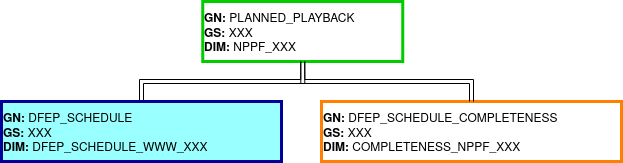
\includegraphics[width=150mm]{../fig/structure_ingestion_dfep_schedule.png}
	\caption{Structure of events inserted by the ingestion module for the MPL\_FS file}
	\label{fg:structure_ingestion_dfep_schedule}
  \end{center}
\end{figure}

The table \ref{tb:description_events_ingestion_dfep_schedule} shows the description of the events inserted by the ingestion.

\begin{landscape}
\begin{longtable}{|M{0.15\linewidth}|M{0.05\linewidth}|M{0.10\linewidth}|M{0.10\linewidth}|M{0.15\linewidth}|M{0.15\linewidth}|M{0.15\linewidth}|}
\hline \textbf{Gauge name} & \textbf{Gauge system} & \textbf{DIM signature} & \textbf{Insertion mode} & \textbf{Description} & \textbf{Start} & \textbf{Stop} \\ \hline
\textbf{DFEP\_SCHEDULE} & XXX & DFEP\_SCHEDULE\_WWW\_XXX & INSERT\_and\_ERASE\_per\_EVENT\_with\_PRIORITY (insert) & Event for representing the \textbf{DFEP schedule} & UTC value inside the start node & UTC value inside the stop node \\ \hline
\textbf{DFEP\_SCHEDULE\_COMPLETENESS} & XXX & \- COMPLETENESS\_NPPF\_XXX & INSERT\_and\_ERASE & Event for representing the \textbf{expectation of the DFEP schedule} & UTC value inside the start node & UTC value inside the stop node \\ \hline
\caption{Table describing the events associated to the ingestion}
\label{tb:description_events_ingestion_dfep_schedule}
\end{longtable}
\end{landscape}

\subsection{Ingestion details}

This section describes some ingestion details for inserting the data. In particular:

\begin{itemize} 

\item The correction of the generation time to avoid overriding data used for completeness analysis
  
\end{itemize}

\subsubsection{Correction of the generation time}

The generation time of the data extracted is one day before the validity start. This could be a problem as the processor of the ORBPRE files could override this data.

To solve this issue the processor changes the generation time to be the validity start.


% Ingestion SRA
\section{Ingestion module for the SRA file}

This sections describes the ingestion module for inserting the SRA information received from the \acrshort{edrs}.

The associated ingestion processor is:

\begin{itemize} 

\item \textbf{s2boa.ingestions.ingestion\_slot\_request\_edrs.ingestion\_slot\_request\_edrs}
  
\end{itemize}

This module uses the following \acrshort{dim} signatures:

\begin{itemize} 

\item \textbf{SLOT\_REQUEST\_EDRS}: data corresponding to the slot request information associated to the EDRS service.

\item \textbf{COMPLETENESS\_NPPF\_XXX}: data corresponding to the definition of planning completeness used for analysis.
  
\end{itemize}

Where XXX is the corresponding satellite ID.

The figure \ref{fg:structure_ingestion_slot_request_edrs} shows a simplified diagram of the structure of events inserted (associated structure of values not included for simplicity).

\begin{figure}[H]
  \begin{center}
	\centering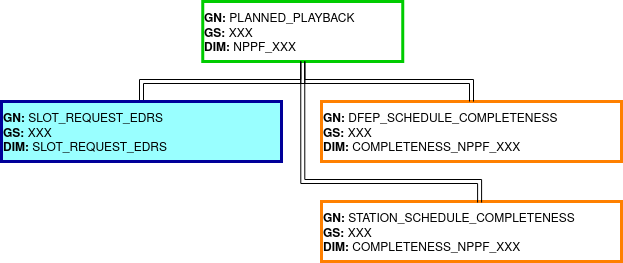
\includegraphics[width=150mm]{../fig/structure_ingestion_slot_request_edrs.png}
	\caption{Structure of events inserted by the ingestion module for the SRA file}
	\label{fg:structure_ingestion_slot_request_edrs}
  \end{center}
\end{figure}

The table \ref{tb:description_events_ingestion_slot_request_edrs} shows the description of the events inserted by the ingestion.

\begin{landscape}
\begin{longtable}{|M{0.15\linewidth}|M{0.05\linewidth}|M{0.10\linewidth}|M{0.10\linewidth}|M{0.15\linewidth}|M{0.15\linewidth}|M{0.15\linewidth}|}
\hline \textbf{Gauge name} & \textbf{Gauge system} & \textbf{DIM signature} & \textbf{Insertion mode} & \textbf{Description} & \textbf{Start} & \textbf{Stop} \\ \hline
\textbf{SLOT\_REQUEST\_EDRS} & XXX & SLOT\_REQUEST\_EDRS & ERASE\_and\_REPLACE\_per\_EVENT (insert) & Event for representing the \textbf{slot request for \acrshort{edrs}} & UTC value inside the Start\_Time node & UTC value inside the Stop\_Time node \\ \hline
\textbf{STATION\_SCHEDULE\_COMPLETENESS} & XXX & \- COMPLETENESS\_NPPF\_XXX & ERASE\_and\_REPLACE (insert\_and\_erase) & Event for representing the \textbf{expectation of the Station schedule} & UTC value inside the Start\_Time node & UTC value inside the Stop\_Time node \\ \hline
\textbf{DFEP\_SCHEDULE\_COMPLETENESS} & XXX & \- COMPLETENESS\_NPPF\_XXX & ERASE\_and\_REPLACE (insert\_and\_erase) & Event for representing the \textbf{expectation of the DFEP schedule} & UTC value inside the Start\_Time node & UTC value inside the Stop\_Time node \\ \hline
\caption{Table describing the events associated to the ingestion}
\label{tb:description_events_ingestion_slot_request_edrs}
\end{longtable}
\end{landscape}


% Ingestion of the REP_PASS_[2|5]
\section{Ingestion module for the REP\_PASS\_[2|5] file}

This sections describes the ingestion module for inserting the \acrshort{dfep} acquisition analysis after reception of data from the satellite.

The associated ingestion processor is:

\begin{itemize} 

\item \textbf{s2boa.ingestions.ingestion\_dfep\_acquisition.ingestion\_dfep\_acquisition}
  
\end{itemize}

This module uses the following \acrshort{dim} signatures:

\begin{itemize} 

\item \textbf{RECEPTION\_XXX}: data corresponding to the acquisition analysis after reception of data from the satellite.

\item \textbf{COMPLETENESS\_NPPF\_XXX}: data corresponding to the definition of planning completeness used for analysis. \textbf{Priority is equal to 30}.

\item \textbf{ISP\_VALIDITY\_PROCESSING\_COMPLETENESS\_XXX}: data corresponding to the definition of \acrshort{isp} processing completeness used for analysis. \textbf{Priority is equal to 10}.

\end{itemize}

Where XXX is the corresponding satellite id, SSS is the station ID and VVV is the \acrshort{vcid} number.

The figure \ref{fg:structure_ingestion_dfep_acquisition} shows a simplified diagram of the structure of events inserted (associated structure of values not included for simplicity).

\begin{figure}[H]
  \begin{center}
	\centering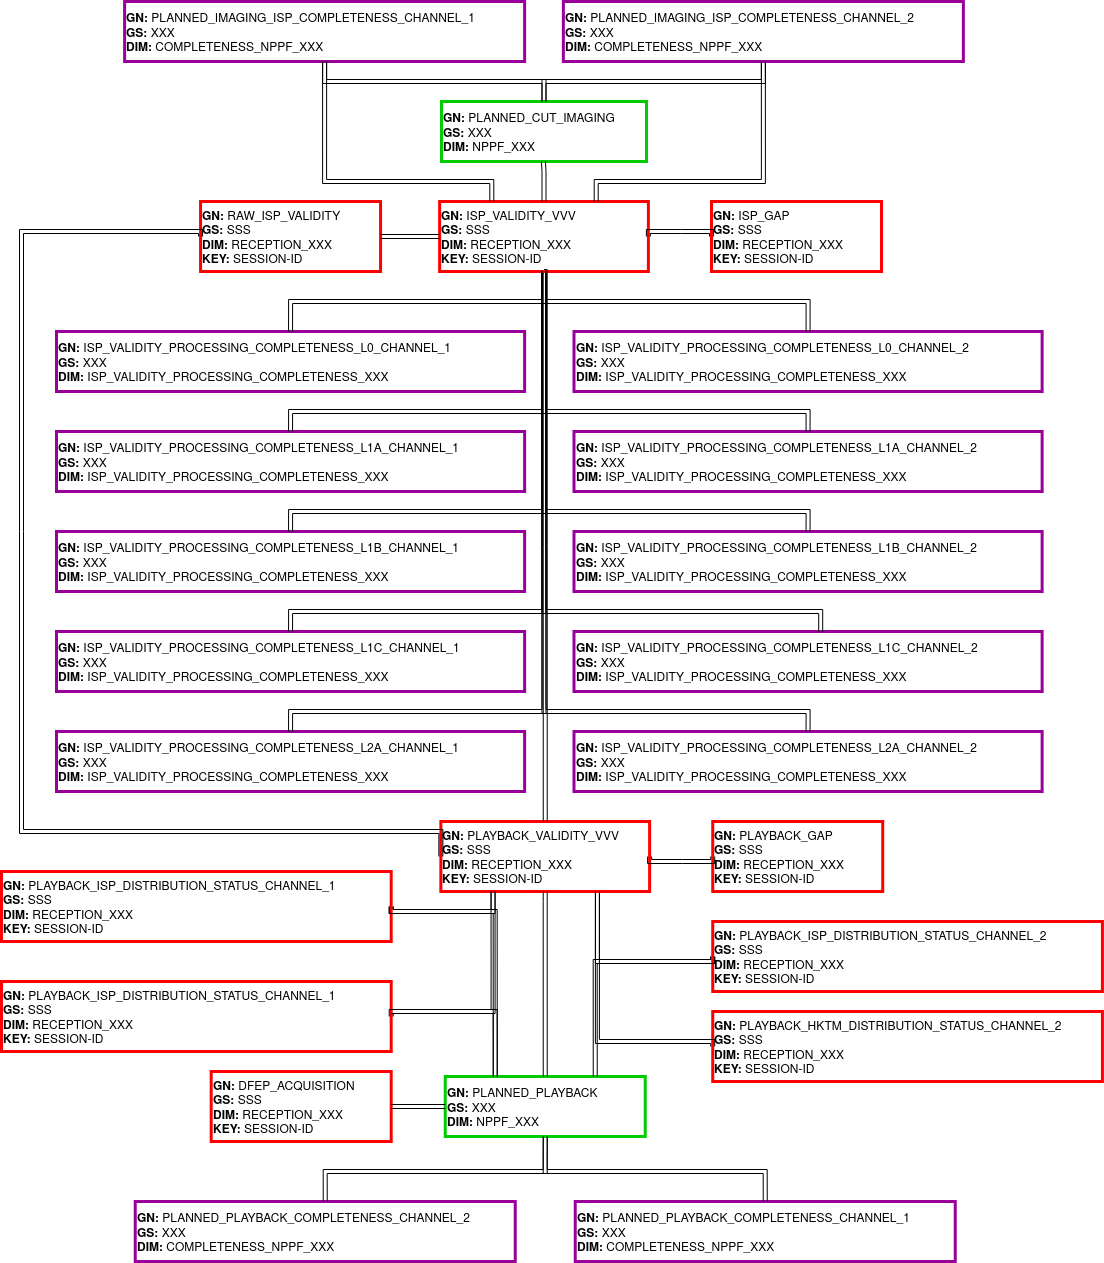
\includegraphics[width=150mm]{../fig/structure_ingestion_dfep_acquisition.png}
	\caption{Structure of events inserted by the ingestion module for the REP\_PASS\_[2|5] file}
	\label{fg:structure_ingestion_dfep_acquisition}
  \end{center}
\end{figure}

The table \ref{tb:description_events_ingestion_dfep_acquisition} shows the description of the events inserted by the ingestion.

\begin{landscape}
\begin{longtable}{|M{0.15\linewidth}|M{0.05\linewidth}|M{0.10\linewidth}|M{0.10\linewidth}|M{0.15\linewidth}|M{0.15\linewidth}|M{0.15\linewidth}|}
\hline \textbf{Gauge name} & \textbf{Gauge system} & \textbf{DIM signature} & \textbf{Insertion mode} & \textbf{Description} & \textbf{Start} & \textbf{Stop} \\ \hline
\textbf{PLAYBACK\_VALIDITY\_VVV} & SSS & \- RECEPTION\_XXX & EVENT\_KEYS (insert) [KEY: SESSION-ID] & Event for representing the \textbf{ground acquisition operation} & UTC time associated to the start of the reception & UTC time associated to the stop of the reception \\ \hline
\textbf{PLAYBACK\_GAP} & SSS & \- RECEPTION\_XXX & EVENT\_KEYS (insert) [KEY: SESSION-ID] & Event for representing a \textbf{gap in the ground acquisition operation} & UTC time associated to the start of the corresponding gap in the reception & UTC time associated to the stop of the corresponding gap in the reception \\ \hline
\textbf{PLANNED\_PLAYBACK\_COMPLETENESS\_CHANNEL\_1} & XXX & \- COMPLETENESS\_NPPF\_XXX & INSERT\_and\_ERASE\_per\_EVENT\_with\_PRIORITY (insert) & Event for completing the \textbf{expectation of the planned playbacks through the channel 1} & Start of the reception through the channel 1 & Stop of the reception through the channel 1 \\ \hline
\textbf{PLANNED\_PLAYBACK\_COMPLETENESS\_CHANNEL\_2} & XXX & \- COMPLETENESS\_NPPF\_XXX & INSERT\_and\_ERASE\_per\_EVENT\_with\_PRIORITY (insert) & Event for completing the \textbf{expectation of the planned playbacks through the channel 2} & Start of the reception through the channel 2 & Stop of the reception through the channel 2 \\ \hline
\textbf{PLANNED\_IMAGING\_ISP\_COMPLETENESS\_CHANNEL\_1} & XXX & \- COMPLETENESS\_NPPF\_XXX & INSERT\_and\_ERASE\_per\_EVENT\_with\_PRIORITY (insert) & Event for completing the \textbf{expectation of the planned imaging sent through the channel 1} & Start of the first received scene thorugh the channel 1 of the corresponding continuous \acrshort{msi} segment & Stop of the last received scene thorugh the channel 1 of the corresponding continuous \acrshort{msi} segment \\ \hline
\textbf{PLANNED\_IMAGING\_ISP\_COMPLETENESS\_CHANNEL\_2} & XXX & \- COMPLETENESS\_NPPF\_XXX & INSERT\_and\_ERASE\_per\_EVENT\_with\_PRIORITY (insert) & Event for completing the \textbf{expectation of the planned imaging sent through the channel 2} & Start of the first received scene thorugh the channel 2 of the corresponding continuous \acrshort{msi} segment & Stop of the last received scene thorugh the channel 2 of the corresponding continuous \acrshort{msi} segment \\ \hline
\textbf{RAW\_ISP\_VALIDITY} & SSS & \- RECEPTION\_XXX & EVENT\_KEYS (insert) [KEY: SESSION-ID] & Event for representing the \textbf{ground acquisition operation} & Start of the first received scene & Stop of the last received scene \\ \hline
\textbf{ISP\_VALIDITY} & SSS & \- RECEPTION\_XXX & EVENT\_KEYS (insert) [KEY: SESSION-ID] & Event for representing the \textbf{ground acquisition operation} & Start of the first received scene of the corresponding continuous \acrshort{msi} segment & Stop of the last received scene of the corresponding continuous \acrshort{msi} segment \\ \hline
\textbf{ISP\_GAP} & SSS & \- RECEPTION\_XXX & EVENT\_KEYS (insert) [KEY: SESSION-ID] & Event for representing a \textbf{gap in the ground acquisition operation} & UTC time associated to the start of the corresponding continuous gap in the received MSI & UTC time associated to the stop of the corresponding continuous gap in the received MSI \\ \hline
\textbf{PLAYBACK\_ISP\_DISTRIBUTION\_STATUS\_CHANNEL\_1} & SSS & \- RECEPTION\_XXX & EVENT\_KEYS (insert) [KEY: SESSION-ID] & Event for representing a \textbf{gap in the ground acquisition operation} & UTC time associated to the start of the \acrshort{msi} reception & UTC time associated to the stop of the \acrshort{msi} reception \\ \hline
\textbf{PLAYBACK\_ISP\_DISTRIBUTION\_STATUS\_CHANNEL\_2} & SSS & \- RECEPTION\_XXX & EVENT\_KEYS (insert) [KEY: SESSION-ID] & Event for representing a \textbf{gap in the ground acquisition operation} & UTC time associated to the start of the \acrshort{msi} reception & UTC time associated to the stop of the \acrshort{msi} reception \\ \hline
\textbf{PLAYBACK\_HKTM\_DISTRIBUTION\_STATUS\_CHANNEL\_1} & SSS & \- RECEPTION\_XXX & EVENT\_KEYS (insert) [KEY: SESSION-ID] & Event for representing a \textbf{gap in the ground acquisition operation} & UTC time associated to the start of the corresponding gap in the \acrshort{hktm} reception & UTC time associated to the stop of the corresponding gap in the \acrshort{hktm} reception \\ \hline
\textbf{PLAYBACK\_HKTM\_DISTRIBUTION\_STATUS\_CHANNEL\_2} & SSS & \- RECEPTION\_XXX & EVENT\_KEYS (insert) [KEY: SESSION-ID] & Event for representing a \textbf{gap in the ground acquisition operation} & UTC time associated to the start of the corresponding gap in the \acrshort{hktm} reception & UTC time associated to the stop of the corresponding gap in the \acrshort{hktm} reception \\ \hline
\textbf{DFEP\_ACQUISITION\_VALIDITY} & SSS & \- RECEPTION\_XXX & EVENT\_KEYS (insert) [KEY: SESSION-ID] & Event for representing a \textbf{gap in the ground acquisition operation} & UTC time associated to the validity start of the received file & UTC time associated to the validity stop of the received file \\ \hline
\textbf{ISP\_VALIDITY\_PROCESSING\_COMPLETENESS\_L0\_CHANNEL\_1} & XXX & \- COMPLETENESS\_NPPF\_XXX & INSERT\_and\_ERASE\_per\_EVENT\_with\_PRIORITY (insert) & Event for representing the \textbf{expectation of the processing of the planned imaging for the L0} & Start of the first received scene of the corresponding continuous \acrshort{msi} segment & Stop of the last received scene of the corresponding continuous \acrshort{msi} segment \\ \hline
\textbf{ISP\_VALIDITY\_PROCESSING\_COMPLETENESS\_L1A\_CHANNEL\_1} & XXX & \- COMPLETENESS\_NPPF\_XXX & INSERT\_and\_ERASE\_per\_EVENT\_with\_PRIORITY (insert) & Event for representing the \textbf{expectation of the processing of the planned imaging for the L0} & Start of the first received scene of the corresponding continuous \acrshort{msi} segment & Stop of the last received scene of the corresponding continuous \acrshort{msi} segment \\ \hline
\textbf{ISP\_VALIDITY\_PROCESSING\_COMPLETENESS\_L1B\_CHANNEL\_1} & XXX & \- COMPLETENESS\_NPPF\_XXX & INSERT\_and\_ERASE\_per\_EVENT\_with\_PRIORITY (insert) & Event for representing the \textbf{expectation of the processing of the planned imaging for the L0} & Start of the first received scene of the corresponding continuous \acrshort{msi} segment & Stop of the last received scene of the corresponding continuous \acrshort{msi} segment \\ \hline
\textbf{ISP\_VALIDITY\_PROCESSING\_COMPLETENESS\_L1C\_CHANNEL\_1} & XXX & \- COMPLETENESS\_NPPF\_XXX & INSERT\_and\_ERASE\_per\_EVENT\_with\_PRIORITY (insert) & Event for representing the \textbf{expectation of the processing of the planned imaging for the L0} & Start of the first received scene of the corresponding continuous \acrshort{msi} segment & Stop of the last received scene of the corresponding continuous \acrshort{msi} segment \\ \hline
\textbf{ISP\_VALIDITY\_PROCESSING\_COMPLETENESS\_L2A\_CHANNEL\_1} & XXX & \- COMPLETENESS\_NPPF\_XXX & INSERT\_and\_ERASE\_per\_EVENT\_with\_PRIORITY (insert) & Event for representing the \textbf{expectation of the processing of the planned imaging for the L0} & Start of the first received scene of the corresponding continuous \acrshort{msi} segment & Stop of the last received scene of the corresponding continuous \acrshort{msi} segment \\ \hline
\textbf{ISP\_VALIDITY\_PROCESSING\_COMPLETENESS\_L0\_CHANNEL\_2} & XXX & \- COMPLETENESS\_NPPF\_XXX & INSERT\_and\_ERASE\_per\_EVENT\_with\_PRIORITY (insert) & Event for representing the \textbf{expectation of the processing of the planned imaging for the L0} & Start of the first received scene of the corresponding continuous \acrshort{msi} segment & Stop of the last received scene of the corresponding continuous \acrshort{msi} segment \\ \hline
\textbf{ISP\_VALIDITY\_PROCESSING\_COMPLETENESS\_L1A\_CHANNEL\_2} & XXX & \- COMPLETENESS\_NPPF\_XXX & INSERT\_and\_ERASE\_per\_EVENT\_with\_PRIORITY (insert) & Event for representing the \textbf{expectation of the processing of the planned imaging for the L0} & Start of the first received scene of the corresponding continuous \acrshort{msi} segment & Stop of the last received scene of the corresponding continuous \acrshort{msi} segment \\ \hline
\textbf{ISP\_VALIDITY\_PROCESSING\_COMPLETENESS\_L1B\_CHANNEL\_2} & XXX & \- COMPLETENESS\_NPPF\_XXX & INSERT\_and\_ERASE\_per\_EVENT\_with\_PRIORITY (insert) & Event for representing the \textbf{expectation of the processing of the planned imaging for the L0} & Start of the first received scene of the corresponding continuous \acrshort{msi} segment & Stop of the last received scene of the corresponding continuous \acrshort{msi} segment \\ \hline
\textbf{ISP\_VALIDITY\_PROCESSING\_COMPLETENESS\_L1C\_CHANNEL\_2} & XXX & \- COMPLETENESS\_NPPF\_XXX & INSERT\_and\_ERASE\_per\_EVENT\_with\_PRIORITY (insert) & Event for representing the \textbf{expectation of the processing of the planned imaging for the L0} & Start of the first received scene of the corresponding continuous \acrshort{msi} segment & Stop of the last received scene of the corresponding continuous \acrshort{msi} segment \\ \hline
\textbf{ISP\_VALIDITY\_PROCESSING\_COMPLETENESS\_L2A\_CHANNEL\_2} & XXX & \- COMPLETENESS\_NPPF\_XXX & INSERT\_and\_ERASE\_per\_EVENT\_with\_PRIORITY (insert) & Event for representing the \textbf{expectation of the processing of the planned imaging for the L0} & Start of the first received scene of the corresponding continuous \acrshort{msi} segment & Stop of the last received scene of the corresponding continuous \acrshort{msi} segment \\ \hline
\caption{Table describing the events associated to the ingestion}
\label{tb:description_events_ingestion_dfep_acquisition}
\end{longtable}
\end{landscape}


% Ingestion of the REP_PASS_E
\section{Ingestion module for the REP\_PASS\_E file}

This sections describes the ingestion module for inserting the \acrshort{efep} acquisition analysis after reception of data from the satellite.

The associated ingestion processor is:

\begin{itemize} 

\item \textbf{s2boa.ingestions.ingestion\_edrs\_acquisition.ingestion\_edrs\_acquisition}

\item \textbf{s2boa.ingestions.ingestion\_vgs\_acquisition.ingestion\_vgs\_acquisition}
  
\end{itemize}

This module uses the following \acrshort{dim} signatures:

\begin{itemize} 

\item \textbf{RECEPTION\_XXX}: data corresponding to the acquisition analysis after reception of data from the satellite.

\item \textbf{COMPLETENESS\_NPPF\_XXX}: data corresponding to the definition of planning completeness used for analysis.

\item \textbf{ISP\_VALIDITY\_PROCESSING\_COMPLETENESS\_XXX}: data corresponding to the definition of \acrshort{isp} processing completeness used for analysis.

\end{itemize}

Where XXX is the corresponding satellite id, SSS is the station ID and VVV is the \acrshort{vcid} number.

The figure \ref{fg:structure_ingestion_eisp} shows a simplified diagram of the structure of events inserted (associated structure of values not included for simplicity).

\begin{figure}[H]
  \begin{center}
	\centering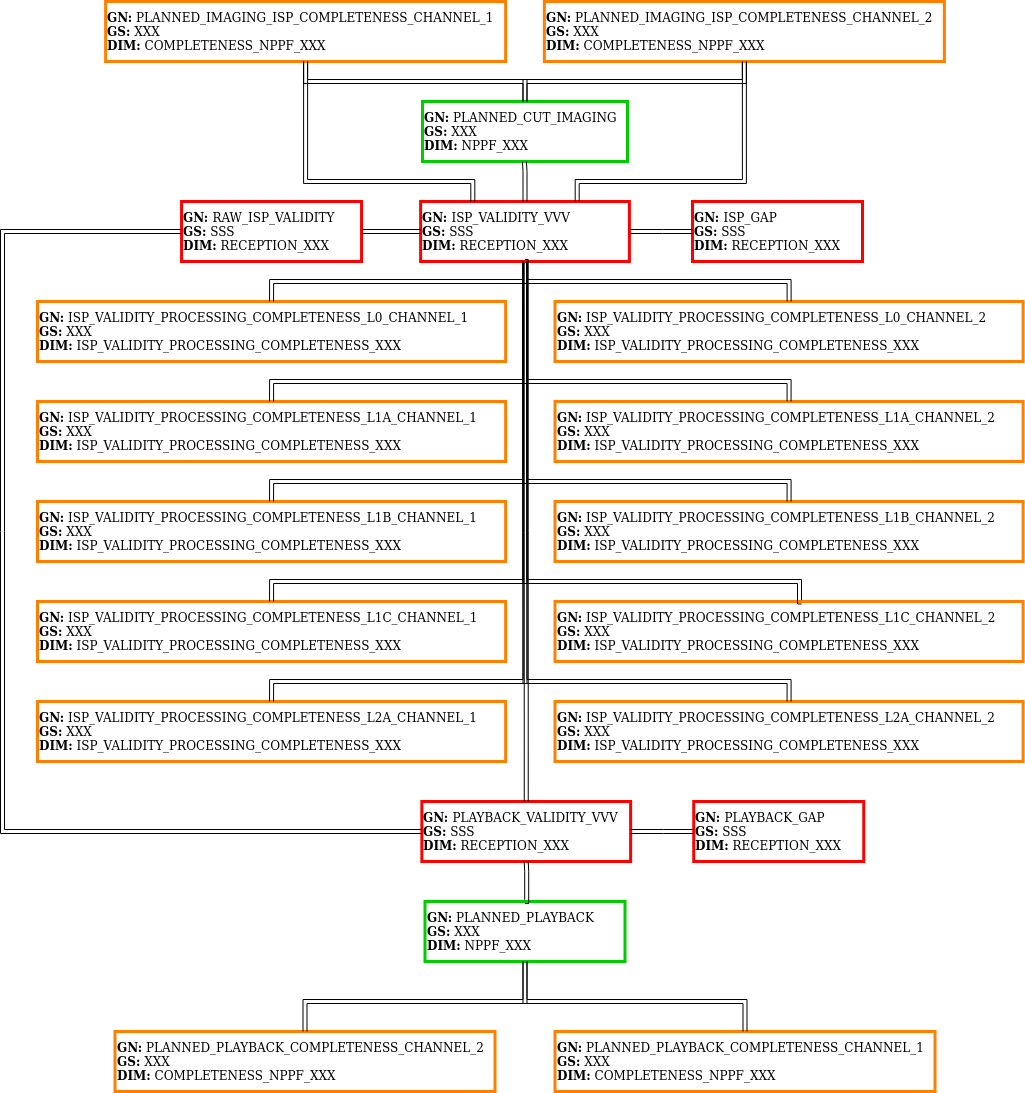
\includegraphics[width=150mm]{../fig/structure_ingestion_eisp.png}
	\caption{Structure of events inserted by the ingestion module for the REP\_PASS\_[2|5] file}
	\label{fg:structure_ingestion_eisp}
  \end{center}
\end{figure}

The table \ref{tb:description_events_ingestion_eisp} shows the description of the events inserted by the ingestion.

\begin{landscape}
\begin{longtable}{|M{0.15\linewidth}|M{0.05\linewidth}|M{0.10\linewidth}|M{0.10\linewidth}|M{0.15\linewidth}|M{0.15\linewidth}|M{0.15\linewidth}|}
\hline \textbf{Gauge name} & \textbf{Gauge system} & \textbf{DIM signature} & \textbf{Insertion mode} & \textbf{Description} & \textbf{Start} & \textbf{Stop} \\ \hline
\textbf{PLAYBACK\_VALIDITY\_VVV} & SSS & \- RECEPTION\_XXX & EVENT\_KEYS (insert) [KEY: SESSION-ID\_CHANNEL\_[1|2]] & Event for representing the \textbf{ground acquisition operation} & UTC time associated to the start of the reception & UTC time associated to the stop of the reception \\ \hline
\textbf{PLAYBACK\_GAP} & SSS & \- RECEPTION\_XXX & EVENT\_KEYS (insert) [KEY: SESSION-ID\_CHANNEL\_[1|2]] & Event for representing a \textbf{gap in the ground acquisition operation} & UTC time associated to the start of the corresponding gap in the reception & UTC time associated to the stop of the corresponding gap in the reception \\ \hline
\textbf{PLANNED\_PLAYBACK\_COMPLETENESS\_CHANNEL\_1} & XXX & \- COMPLETENESS\_NPPF\_XXX & ERASE\_and\_REPLACE\_per\_EVENT (insert) & Event for completing the \textbf{expectation of the planned playbacks through the channel 1} & Start of the reception through the channel 1 & Stop of the reception through the channel 1 \\ \hline
\textbf{PLANNED\_PLAYBACK\_COMPLETENESS\_CHANNEL\_2} & XXX & \- COMPLETENESS\_NPPF\_XXX & ERASE\_and\_REPLACE\_per\_EVENT (insert) & Event for completing the \textbf{expectation of the planned playbacks through the channel 2} & Start of the reception through the channel 2 & Stop of the reception through the channel 2 \\ \hline
\textbf{PLANNED\_IMAGING\_ISP\_COMPLETENESS\_CHANNEL\_1} & XXX & \- COMPLETENESS\_NPPF\_XXX & ERASE\_and\_REPLACE\_per\_EVENT (insert) & Event for completing the \textbf{expectation of the planned imaging sent through the channel 1} & Start of the first received scene thorugh the channel 1 of the corresponding continuous \acrshort{msi} segment & Stop of the last received scene thorugh the channel 1 of the corresponding continuous \acrshort{msi} segment \\ \hline
\textbf{PLANNED\_IMAGING\_ISP\_COMPLETENESS\_CHANNEL\_2} & XXX & \- COMPLETENESS\_NPPF\_XXX & ERASE\_and\_REPLACE\_per\_EVENT (insert) & Event for completing the \textbf{expectation of the planned imaging sent through the channel 2} & Start of the first received scene thorugh the channel 2 of the corresponding continuous \acrshort{msi} segment & Stop of the last received scene thorugh the channel 2 of the corresponding continuous \acrshort{msi} segment \\ \hline
\textbf{RAW\_ISP\_VALIDITY} & SSS & \- RECEPTION\_XXX & EVENT\_KEYS (insert) [KEY: SESSION-ID\_CHANNEL\_[1|2]] & Event for representing the \textbf{ground acquisition operation} & Start of the first received scene & Stop of the last received scene \\ \hline
\textbf{ISP\_VALIDITY} & SSS & \- RECEPTION\_XXX & EVENT\_KEYS (insert) [KEY: SESSION-ID\_CHANNEL\_[1|2]] & Event for representing the \textbf{ground acquisition operation} & Start of the first received scene of the corresponding continuous \acrshort{msi} segment & Stop of the last received scene of the corresponding continuous \acrshort{msi} segment \\ \hline
\textbf{ISP\_GAP} & SSS & \- RECEPTION\_XXX & EVENT\_KEYS (insert) [KEY: SESSION-ID\_CHANNEL\_[1|2]] & Event for representing a \textbf{gap in the ground acquisition operation} & UTC time associated to the start of the corresponding continuous gap in the received MSI & UTC time associated to the stop of the corresponding continuous gap in the received MSI \\ \hline
\textbf{ISP\_VALIDITY\_PROCESSING\_COMPLETENESS\_L0\_CHANNEL\_1} & XXX & \- COMPLETENESS\_NPPF\_XXX & ERASE\_and\_REPLACE\_per\_EVENT (insert) & Event for representing the \textbf{expectation of the processing of the planned imaging for the L0} & Start of the first received scene of the corresponding continuous \acrshort{msi} segment & Stop of the last received scene of the corresponding continuous \acrshort{msi} segment \\ \hline
\textbf{ISP\_VALIDITY\_PROCESSING\_COMPLETENESS\_L1A\_CHANNEL\_1} & XXX & \- COMPLETENESS\_NPPF\_XXX & ERASE\_and\_REPLACE\_per\_EVENT (insert) & Event for representing the \textbf{expectation of the processing of the planned imaging for the L0} & Start of the first received scene of the corresponding continuous \acrshort{msi} segment & Stop of the last received scene of the corresponding continuous \acrshort{msi} segment \\ \hline
\textbf{ISP\_VALIDITY\_PROCESSING\_COMPLETENESS\_L1B\_CHANNEL\_1} & XXX & \- COMPLETENESS\_NPPF\_XXX & ERASE\_and\_REPLACE\_per\_EVENT (insert) & Event for representing the \textbf{expectation of the processing of the planned imaging for the L0} & Start of the first received scene of the corresponding continuous \acrshort{msi} segment & Stop of the last received scene of the corresponding continuous \acrshort{msi} segment \\ \hline
\textbf{ISP\_VALIDITY\_PROCESSING\_COMPLETENESS\_L1C\_CHANNEL\_1} & XXX & \- COMPLETENESS\_NPPF\_XXX & ERASE\_and\_REPLACE\_per\_EVENT (insert) & Event for representing the \textbf{expectation of the processing of the planned imaging for the L0} & Start of the first received scene of the corresponding continuous \acrshort{msi} segment & Stop of the last received scene of the corresponding continuous \acrshort{msi} segment \\ \hline
\textbf{ISP\_VALIDITY\_PROCESSING\_COMPLETENESS\_L2A\_CHANNEL\_1} & XXX & \- COMPLETENESS\_NPPF\_XXX & ERASE\_and\_REPLACE\_per\_EVENT (insert) & Event for representing the \textbf{expectation of the processing of the planned imaging for the L0} & Start of the first received scene of the corresponding continuous \acrshort{msi} segment & Stop of the last received scene of the corresponding continuous \acrshort{msi} segment \\ \hline
\textbf{ISP\_VALIDITY\_PROCESSING\_COMPLETENESS\_L0\_CHANNEL\_2} & XXX & \- COMPLETENESS\_NPPF\_XXX & ERASE\_and\_REPLACE\_per\_EVENT (insert) & Event for representing the \textbf{expectation of the processing of the planned imaging for the L0} & Start of the first received scene of the corresponding continuous \acrshort{msi} segment & Stop of the last received scene of the corresponding continuous \acrshort{msi} segment \\ \hline
\textbf{ISP\_VALIDITY\_PROCESSING\_COMPLETENESS\_L1A\_CHANNEL\_2} & XXX & \- COMPLETENESS\_NPPF\_XXX & ERASE\_and\_REPLACE\_per\_EVENT (insert) & Event for representing the \textbf{expectation of the processing of the planned imaging for the L0} & Start of the first received scene of the corresponding continuous \acrshort{msi} segment & Stop of the last received scene of the corresponding continuous \acrshort{msi} segment \\ \hline
\textbf{ISP\_VALIDITY\_PROCESSING\_COMPLETENESS\_L1B\_CHANNEL\_2} & XXX & \- COMPLETENESS\_NPPF\_XXX & ERASE\_and\_REPLACE\_per\_EVENT (insert) & Event for representing the \textbf{expectation of the processing of the planned imaging for the L0} & Start of the first received scene of the corresponding continuous \acrshort{msi} segment & Stop of the last received scene of the corresponding continuous \acrshort{msi} segment \\ \hline
\textbf{ISP\_VALIDITY\_PROCESSING\_COMPLETENESS\_L1C\_CHANNEL\_2} & XXX & \- COMPLETENESS\_NPPF\_XXX & ERASE\_and\_REPLACE\_per\_EVENT (insert) & Event for representing the \textbf{expectation of the processing of the planned imaging for the L0} & Start of the first received scene of the corresponding continuous \acrshort{msi} segment & Stop of the last received scene of the corresponding continuous \acrshort{msi} segment \\ \hline
\textbf{ISP\_VALIDITY\_PROCESSING\_COMPLETENESS\_L2A\_CHANNEL\_2} & XXX & \- COMPLETENESS\_NPPF\_XXX & ERASE\_and\_REPLACE\_per\_EVENT (insert) & Event for representing the \textbf{expectation of the processing of the planned imaging for the L0} & Start of the first received scene of the corresponding continuous \acrshort{msi} segment & Stop of the last received scene of the corresponding continuous \acrshort{msi} segment \\ \hline
\caption{Table describing the events associated to the ingestion}
\label{tb:description_events_ingestion_eisp}
\end{longtable}
\end{landscape}


% Ingestion of the REP_OPDPC
\section{Ingestion module for the REP\_OPDPC file}

This sections describes the ingestion module for inserting the \acrshort{dpc} processing analysis.

The associated ingestion processor is:

\begin{itemize} 

\item \textbf{s2boa.ingestions.ingestion\_dpc.ingestion\_dpc}
  
\end{itemize}

This module uses the following \acrshort{dim} signatures:

\begin{itemize} 

\item \textbf{PROCESSING\_XXX}: data corresponding to the processing analysis.

\item \textbf{COMPLETENESS\_NPPF\_XXX}: data corresponding to the definition of planning completeness used for analysis.

\item \textbf{ISP\_VALIDITY\_PROCESSING\_COMPLETENESS\_XXX}: data corresponding to the definition of \acrshort{isp} processing completeness used for analysis.

\item \textbf{INDEXING\_XXX}: data corresponding to the indexing analysis of products.

\item \textbf{ARCHIVING}: data corresponding to the archiving analysis of products.

\item \textbf{CATALOGING}: data corresponding to the cataloging analysis of products.

\item \textbf{LONG\_TERM\_ARCHIVING}: data corresponding to the cataloging analysis of products.

\end{itemize}

Where XXX is the corresponding satellite id.

The figure \ref{fg:structure_ingestion_dpc_events} shows a simplified diagram of the structure of events inserted (associated structure of values not included for simplicity).

\begin{figure}[H]
  \begin{center}
	\centering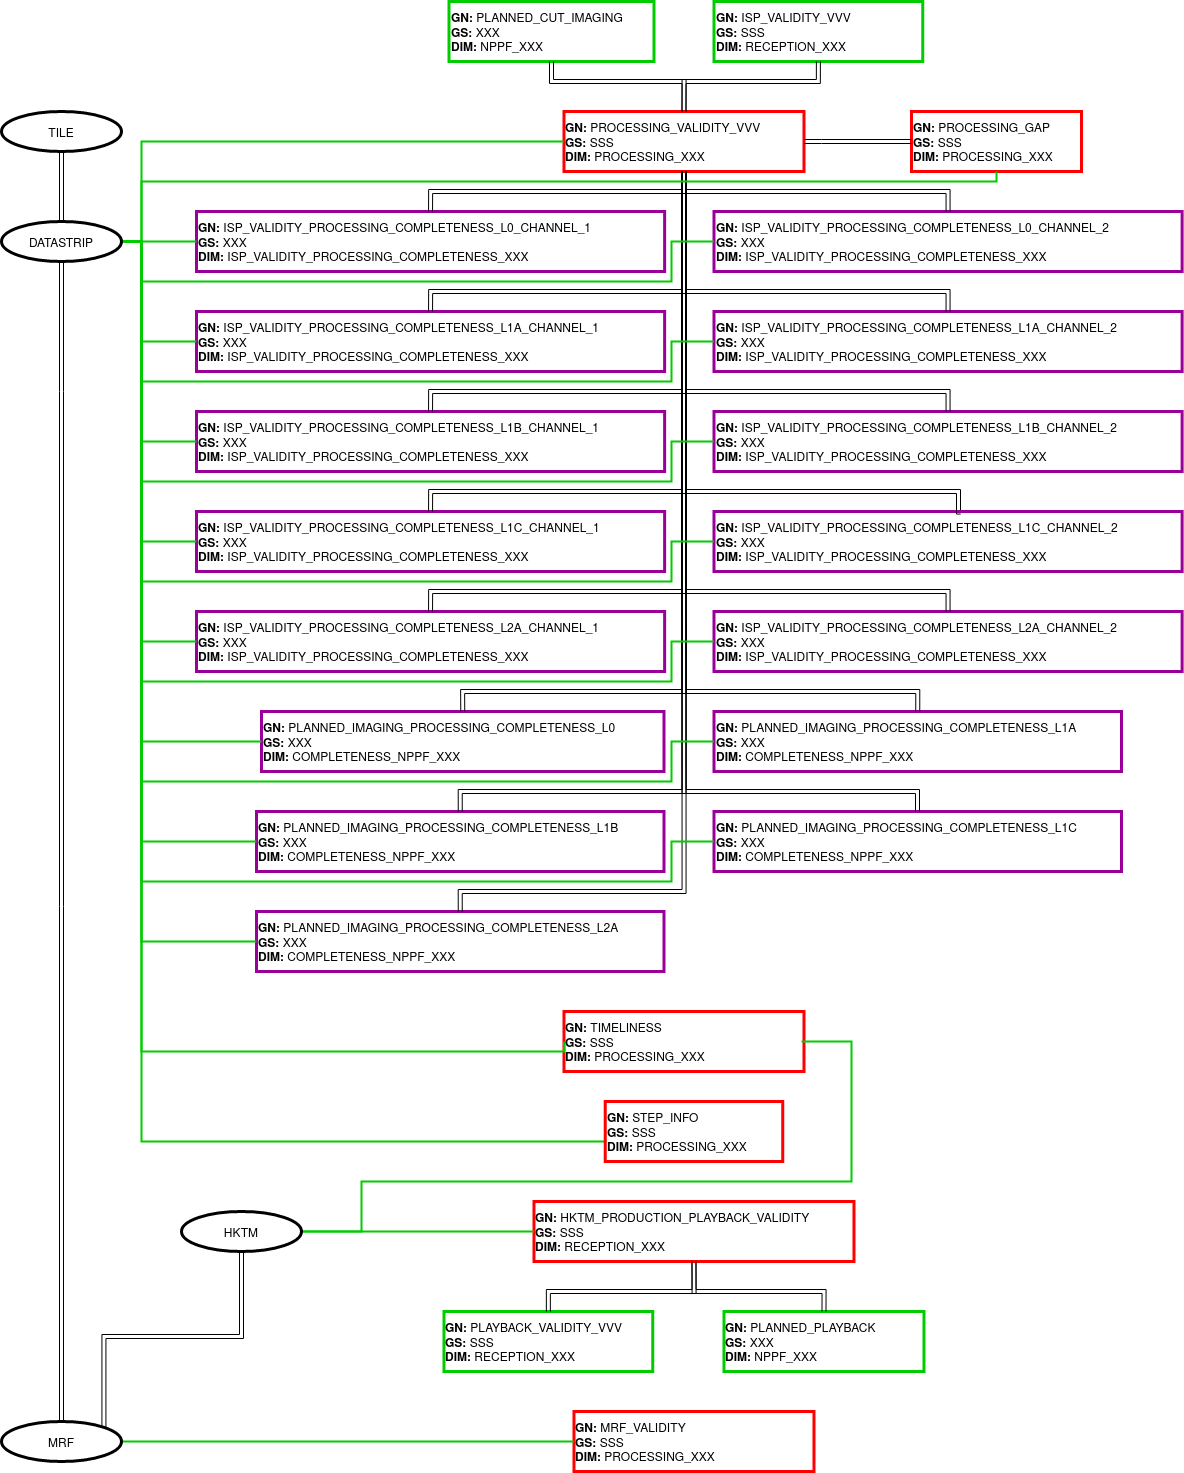
\includegraphics[width=150mm]{../fig/structure_ingestion_dpc_events.png}
	\caption{Structure of events inserted by the ingestion module for the REP\_OPDPC file}
	\label{fg:structure_ingestion_dpc_events}
  \end{center}
\end{figure}

The table \ref{tb:description_events_ingestion_dpc} shows the description of the events inserted by the ingestion.

\begin{landscape}
\begin{longtable}{|M{0.15\linewidth}|M{0.05\linewidth}|M{0.10\linewidth}|M{0.10\linewidth}|M{0.15\linewidth}|M{0.15\linewidth}|M{0.15\linewidth}|}
\hline \textbf{Gauge name} & \textbf{Gauge system} & \textbf{DIM signature} & \textbf{Insertion mode} & \textbf{Description} & \textbf{Start} & \textbf{Stop} \\ \hline
\textbf{PLAYBACK\_VALIDITY\_VVV} & SSS & \- RECEPTION\_XXX & EVENT\_KEYS (insert) & Event for representing the \textbf{ground acquisition operation} & UTC time associated to the start of the reception & UTC time associated to the stop of the reception \\ \hline
\textbf{PLAYBACK\_GAP} & SSS & \- RECEPTION\_XXX & EVENT\_KEYS (insert) & Event for representing a \textbf{gap in the ground acquisition operation} & UTC time associated to the start of the corresponding gap in the reception & UTC time associated to the stop of the corresponding gap in the reception \\ \hline
\textbf{PLANNED\_PLAYBACK\_COMPLETENESS\_CHANNEL\_1} & XXX & \- COMPLETENESS\_NPPF\_XXX & ERASE\_and\_REPLACE\_per\_EVENT (insert) & Event for completing the \textbf{expectation of the planned playbacks through the channel 1} & Start of the reception through the channel 1 & Stop of the reception through the channel 1 \\ \hline
\textbf{PLANNED\_PLAYBACK\_COMPLETENESS\_CHANNEL\_2} & XXX & \- COMPLETENESS\_NPPF\_XXX & ERASE\_and\_REPLACE\_per\_EVENT (insert) & Event for completing the \textbf{expectation of the planned playbacks through the channel 2} & Start of the reception through the channel 2 & Stop of the reception through the channel 2 \\ \hline
\textbf{PLANNED\_IMAGING\_ISP\_COMPLETENESS\_CHANNEL\_1} & XXX & \- COMPLETENESS\_NPPF\_XXX & ERASE\_and\_REPLACE\_per\_EVENT (insert) & Event for completing the \textbf{expectation of the planned imaging sent through the channel 1} & Start of the first received scene thorugh the channel 1 of the corresponding continuous \acrshort{msi} segment & Stop of the last received scene thorugh the channel 1 of the corresponding continuous \acrshort{msi} segment \\ \hline
\textbf{PLANNED\_IMAGING\_ISP\_COMPLETENESS\_CHANNEL\_2} & XXX & \- COMPLETENESS\_NPPF\_XXX & ERASE\_and\_REPLACE\_per\_EVENT (insert) & Event for completing the \textbf{expectation of the planned imaging sent through the channel 2} & Start of the first received scene thorugh the channel 2 of the corresponding continuous \acrshort{msi} segment & Stop of the last received scene thorugh the channel 2 of the corresponding continuous \acrshort{msi} segment \\ \hline
\textbf{RAW\_ISP\_VALIDITY} & SSS & \- RECEPTION\_XXX & EVENT\_KEYS (insert) & Event for representing the \textbf{ground acquisition operation} & Start of the first received scene & Stop of the last received scene \\ \hline
\textbf{ISP\_VALIDITY} & SSS & \- RECEPTION\_XXX & EVENT\_KEYS (insert) & Event for representing the \textbf{ground acquisition operation} & Start of the first received scene of the corresponding continuous \acrshort{msi} segment & Stop of the last received scene of the corresponding continuous \acrshort{msi} segment \\ \hline
\textbf{ISP\_GAP} & SSS & \- RECEPTION\_XXX & EVENT\_KEYS (insert) & Event for representing a \textbf{gap in the ground acquisition operation} & UTC time associated to the start of the corresponding continuous gap in the received MSI & UTC time associated to the stop of the corresponding continuous gap in the received MSI \\ \hline
\textbf{PLAYBACK\_ISP\_DISTRIBUTION\_STATUS\_CHANNEL\_1} & SSS & \- RECEPTION\_XXX & EVENT\_KEYS (insert) & Event for representing a \textbf{gap in the ground acquisition operation} & UTC time associated to the start of the \acrshort{msi} reception & UTC time associated to the stop of the \acrshort{msi} reception \\ \hline
\textbf{PLAYBACK\_ISP\_DISTRIBUTION\_STATUS\_CHANNEL\_2} & SSS & \- RECEPTION\_XXX & EVENT\_KEYS (insert) & Event for representing a \textbf{gap in the ground acquisition operation} & UTC time associated to the start of the \acrshort{msi} reception & UTC time associated to the stop of the \acrshort{msi} reception \\ \hline
\textbf{PLAYBACK\_HKTM\_DISTRIBUTION\_STATUS\_CHANNEL\_1} & SSS & \- RECEPTION\_XXX & EVENT\_KEYS (insert) & Event for representing a \textbf{gap in the ground acquisition operation} & UTC time associated to the start of the corresponding gap in the \acrshort{hktm} reception & UTC time associated to the stop of the corresponding gap in the \acrshort{hktm} reception \\ \hline
\textbf{PLAYBACK\_HKTM\_DISTRIBUTION\_STATUS\_CHANNEL\_2} & SSS & \- RECEPTION\_XXX & EVENT\_KEYS (insert) & Event for representing a \textbf{gap in the ground acquisition operation} & UTC time associated to the start of the corresponding gap in the \acrshort{hktm} reception & UTC time associated to the stop of the corresponding gap in the \acrshort{hktm} reception \\ \hline
\textbf{DFEP\_ACQUISITION\_VALIDITY} & SSS & \- RECEPTION\_XXX & EVENT\_KEYS (insert) & Event for representing a \textbf{gap in the ground acquisition operation} & UTC time associated to the validity start of the received file & UTC time associated to the validity stop of the received file \\ \hline
\textbf{ISP\_VALIDITY\_PROCESSING\_COMPLETENESS\_L0\_CHANNEL\_1} & XXX & \- COMPLETENESS\_NPPF\_XXX & ERASE\_and\_REPLACE\_per\_EVENT (insert) & Event for representing the \textbf{expectation of the processing of the planned imaging for the L0} & Start of the first received scene of the corresponding continuous \acrshort{msi} segment & Stop of the last received scene of the corresponding continuous \acrshort{msi} segment \\ \hline
\textbf{ISP\_VALIDITY\_PROCESSING\_COMPLETENESS\_L1A\_CHANNEL\_1} & XXX & \- COMPLETENESS\_NPPF\_XXX & ERASE\_and\_REPLACE\_per\_EVENT (insert) & Event for representing the \textbf{expectation of the processing of the planned imaging for the L0} & Start of the first received scene of the corresponding continuous \acrshort{msi} segment & Stop of the last received scene of the corresponding continuous \acrshort{msi} segment \\ \hline
\textbf{ISP\_VALIDITY\_PROCESSING\_COMPLETENESS\_L1B\_CHANNEL\_1} & XXX & \- COMPLETENESS\_NPPF\_XXX & ERASE\_and\_REPLACE\_per\_EVENT (insert) & Event for representing the \textbf{expectation of the processing of the planned imaging for the L0} & Start of the first received scene of the corresponding continuous \acrshort{msi} segment & Stop of the last received scene of the corresponding continuous \acrshort{msi} segment \\ \hline
\textbf{ISP\_VALIDITY\_PROCESSING\_COMPLETENESS\_L1C\_CHANNEL\_1} & XXX & \- COMPLETENESS\_NPPF\_XXX & ERASE\_and\_REPLACE\_per\_EVENT (insert) & Event for representing the \textbf{expectation of the processing of the planned imaging for the L0} & Start of the first received scene of the corresponding continuous \acrshort{msi} segment & Stop of the last received scene of the corresponding continuous \acrshort{msi} segment \\ \hline
\textbf{ISP\_VALIDITY\_PROCESSING\_COMPLETENESS\_L2A\_CHANNEL\_1} & XXX & \- COMPLETENESS\_NPPF\_XXX & ERASE\_and\_REPLACE\_per\_EVENT (insert) & Event for representing the \textbf{expectation of the processing of the planned imaging for the L0} & Start of the first received scene of the corresponding continuous \acrshort{msi} segment & Stop of the last received scene of the corresponding continuous \acrshort{msi} segment \\ \hline
\textbf{ISP\_VALIDITY\_PROCESSING\_COMPLETENESS\_L0\_CHANNEL\_2} & XXX & \- COMPLETENESS\_NPPF\_XXX & ERASE\_and\_REPLACE\_per\_EVENT (insert) & Event for representing the \textbf{expectation of the processing of the planned imaging for the L0} & Start of the first received scene of the corresponding continuous \acrshort{msi} segment & Stop of the last received scene of the corresponding continuous \acrshort{msi} segment \\ \hline
\textbf{ISP\_VALIDITY\_PROCESSING\_COMPLETENESS\_L1A\_CHANNEL\_2} & XXX & \- COMPLETENESS\_NPPF\_XXX & ERASE\_and\_REPLACE\_per\_EVENT (insert) & Event for representing the \textbf{expectation of the processing of the planned imaging for the L0} & Start of the first received scene of the corresponding continuous \acrshort{msi} segment & Stop of the last received scene of the corresponding continuous \acrshort{msi} segment \\ \hline
\textbf{ISP\_VALIDITY\_PROCESSING\_COMPLETENESS\_L1B\_CHANNEL\_2} & XXX & \- COMPLETENESS\_NPPF\_XXX & ERASE\_and\_REPLACE\_per\_EVENT (insert) & Event for representing the \textbf{expectation of the processing of the planned imaging for the L0} & Start of the first received scene of the corresponding continuous \acrshort{msi} segment & Stop of the last received scene of the corresponding continuous \acrshort{msi} segment \\ \hline
\textbf{ISP\_VALIDITY\_PROCESSING\_COMPLETENESS\_L1C\_CHANNEL\_2} & XXX & \- COMPLETENESS\_NPPF\_XXX & ERASE\_and\_REPLACE\_per\_EVENT (insert) & Event for representing the \textbf{expectation of the processing of the planned imaging for the L0} & Start of the first received scene of the corresponding continuous \acrshort{msi} segment & Stop of the last received scene of the corresponding continuous \acrshort{msi} segment \\ \hline
\textbf{ISP\_VALIDITY\_PROCESSING\_COMPLETENESS\_L2A\_CHANNEL\_2} & XXX & \- COMPLETENESS\_NPPF\_XXX & ERASE\_and\_REPLACE\_per\_EVENT (insert) & Event for representing the \textbf{expectation of the processing of the planned imaging for the L0} & Start of the first received scene of the corresponding continuous \acrshort{msi} segment & Stop of the last received scene of the corresponding continuous \acrshort{msi} segment \\ \hline
\caption{Table describing the events associated to the ingestion}
\label{tb:description_events_ingestion_dpc}
\end{longtable}
\end{landscape}

The figure \ref{fg:structure_ingestion_dpc_annotations} shows a simplified diagram of the structure of annotations inserted (associated structure of values not included for simplicity).

\begin{figure}[H]
  \begin{center}
	\centering\includegraphics[width=150mm]{../fig/structure_ingestion_dpc_annotations.png}
	\caption{Structure of annotations inserted by the ingestion module for the REP\_OPDPC file}
	\label{fg:structure_ingestion_dpc_annotations}
  \end{center}
\end{figure}



% Insert automatically generated code of s2boa
\chapter{Ingestion modules code documentation}
\section{Subpackages}
\label{\detokenize{s2boa:subpackages}}

\subsection{s2boa.ingestions package}
\label{\detokenize{s2boa.ingestions:s2boa-ingestions-package}}\label{\detokenize{s2boa.ingestions::doc}}

\subsubsection{Submodules}
\label{\detokenize{s2boa.ingestions:submodules}}

\subsubsection{s2boa.ingestions.ingestion\_ai.ingestion\_ai module}
\label{\detokenize{s2boa.ingestions:module-s2boa.ingestions.ingestion_ai.ingestion_ai}}\label{\detokenize{s2boa.ingestions:s2boa-ingestions-ingestion-ai-ingestion-ai-module}}\index{module@\spxentry{module}!s2boa.ingestions.ingestion\_ai.ingestion\_ai@\spxentry{s2boa.ingestions.ingestion\_ai.ingestion\_ai}}\index{s2boa.ingestions.ingestion\_ai.ingestion\_ai@\spxentry{s2boa.ingestions.ingestion\_ai.ingestion\_ai}!module@\spxentry{module}}
Ingestion module for the REP\_OPAI files of Sentinel\sphinxhyphen{}2

Written by DEIMOS Space S.L. (femd)

module eboa
\index{process\_file() (in module s2boa.ingestions.ingestion\_ai.ingestion\_ai)@\spxentry{process\_file()}\spxextra{in module s2boa.ingestions.ingestion\_ai.ingestion\_ai}}

\begin{fulllineitems}
\phantomsection\label{\detokenize{s2boa.ingestions:s2boa.ingestions.ingestion_ai.ingestion_ai.process_file}}\pysiglinewithargsret{\sphinxcode{\sphinxupquote{s2boa.ingestions.ingestion\_ai.ingestion\_ai.}}\sphinxbfcode{\sphinxupquote{process\_file}}}{\emph{\DUrole{n}{file\_path}}, \emph{\DUrole{n}{engine}}, \emph{\DUrole{n}{query}}, \emph{\DUrole{n}{reception\_time}}}{}
Function to process the file and insert its relevant information
into the DDBB of the eboa
\begin{quote}\begin{description}
\item[{Parameters}] \leavevmode\begin{itemize}
\item {} 
\sphinxstyleliteralstrong{\sphinxupquote{file\_path}} (\sphinxstyleliteralemphasis{\sphinxupquote{str}}) \textendash{} path to the file to be processed

\item {} 
\sphinxstyleliteralstrong{\sphinxupquote{engine}} (\sphinxstyleliteralemphasis{\sphinxupquote{Engine}}) \textendash{} Engine instance

\item {} 
\sphinxstyleliteralstrong{\sphinxupquote{query}} (\sphinxstyleliteralemphasis{\sphinxupquote{Query}}) \textendash{} Query instance

\item {} 
\sphinxstyleliteralstrong{\sphinxupquote{reception\_time}} (\sphinxstyleliteralemphasis{\sphinxupquote{str}}) \textendash{} time of the reception of the file by the triggering

\end{itemize}

\end{description}\end{quote}

\end{fulllineitems}



\subsubsection{s2boa.ingestions.ingestion\_dam.ingestion\_dam module}
\label{\detokenize{s2boa.ingestions:module-s2boa.ingestions.ingestion_dam.ingestion_dam}}\label{\detokenize{s2boa.ingestions:s2boa-ingestions-ingestion-dam-ingestion-dam-module}}\index{module@\spxentry{module}!s2boa.ingestions.ingestion\_dam.ingestion\_dam@\spxentry{s2boa.ingestions.ingestion\_dam.ingestion\_dam}}\index{s2boa.ingestions.ingestion\_dam.ingestion\_dam@\spxentry{s2boa.ingestions.ingestion\_dam.ingestion\_dam}!module@\spxentry{module}}
Ingestion module for the REP\_OPDAM files of Sentinel\sphinxhyphen{}2

Written by DEIMOS Space S.L. (femd)

module eboa
\index{process\_file() (in module s2boa.ingestions.ingestion\_dam.ingestion\_dam)@\spxentry{process\_file()}\spxextra{in module s2boa.ingestions.ingestion\_dam.ingestion\_dam}}

\begin{fulllineitems}
\phantomsection\label{\detokenize{s2boa.ingestions:s2boa.ingestions.ingestion_dam.ingestion_dam.process_file}}\pysiglinewithargsret{\sphinxcode{\sphinxupquote{s2boa.ingestions.ingestion\_dam.ingestion\_dam.}}\sphinxbfcode{\sphinxupquote{process\_file}}}{\emph{\DUrole{n}{file\_path}}, \emph{\DUrole{n}{engine}}, \emph{\DUrole{n}{query}}, \emph{\DUrole{n}{reception\_time}}}{}
Function to process the file and insert its relevant information
into the DDBB of the eboa
\begin{quote}\begin{description}
\item[{Parameters}] \leavevmode\begin{itemize}
\item {} 
\sphinxstyleliteralstrong{\sphinxupquote{file\_path}} (\sphinxstyleliteralemphasis{\sphinxupquote{str}}) \textendash{} path to the file to be processed

\item {} 
\sphinxstyleliteralstrong{\sphinxupquote{engine}} (\sphinxstyleliteralemphasis{\sphinxupquote{Engine}}) \textendash{} Engine instance

\item {} 
\sphinxstyleliteralstrong{\sphinxupquote{query}} (\sphinxstyleliteralemphasis{\sphinxupquote{Query}}) \textendash{} Query instance

\item {} 
\sphinxstyleliteralstrong{\sphinxupquote{reception\_time}} (\sphinxstyleliteralemphasis{\sphinxupquote{str}}) \textendash{} time of the reception of the file by the triggering

\end{itemize}

\end{description}\end{quote}

\end{fulllineitems}



\subsubsection{s2boa.ingestions.ingestion\_dfep\_acquisition.ingestion\_dfep\_acquisition module}
\label{\detokenize{s2boa.ingestions:module-s2boa.ingestions.ingestion_dfep_acquisition.ingestion_dfep_acquisition}}\label{\detokenize{s2boa.ingestions:s2boa-ingestions-ingestion-dfep-acquisition-ingestion-dfep-acquisition-module}}\index{module@\spxentry{module}!s2boa.ingestions.ingestion\_dfep\_acquisition.ingestion\_dfep\_acquisition@\spxentry{s2boa.ingestions.ingestion\_dfep\_acquisition.ingestion\_dfep\_acquisition}}\index{s2boa.ingestions.ingestion\_dfep\_acquisition.ingestion\_dfep\_acquisition@\spxentry{s2boa.ingestions.ingestion\_dfep\_acquisition.ingestion\_dfep\_acquisition}!module@\spxentry{module}}
Ingestion module for the REP\_PASS\_2|5 files of Sentinel\sphinxhyphen{}2

Written by DEIMOS Space S.L. (dibb)

module eboa
\index{process\_file() (in module s2boa.ingestions.ingestion\_dfep\_acquisition.ingestion\_dfep\_acquisition)@\spxentry{process\_file()}\spxextra{in module s2boa.ingestions.ingestion\_dfep\_acquisition.ingestion\_dfep\_acquisition}}

\begin{fulllineitems}
\phantomsection\label{\detokenize{s2boa.ingestions:s2boa.ingestions.ingestion_dfep_acquisition.ingestion_dfep_acquisition.process_file}}\pysiglinewithargsret{\sphinxcode{\sphinxupquote{s2boa.ingestions.ingestion\_dfep\_acquisition.ingestion\_dfep\_acquisition.}}\sphinxbfcode{\sphinxupquote{process\_file}}}{\emph{\DUrole{n}{file\_path}}, \emph{\DUrole{n}{engine}}, \emph{\DUrole{n}{query}}, \emph{\DUrole{n}{reception\_time}}}{}
Function to process the file and insert its relevant information
into the DDBB of the eboa
\begin{quote}\begin{description}
\item[{Parameters}] \leavevmode\begin{itemize}
\item {} 
\sphinxstyleliteralstrong{\sphinxupquote{file\_path}} (\sphinxstyleliteralemphasis{\sphinxupquote{str}}) \textendash{} path to the file to be processed

\item {} 
\sphinxstyleliteralstrong{\sphinxupquote{engine}} (\sphinxstyleliteralemphasis{\sphinxupquote{Engine}}) \textendash{} Engine instance

\item {} 
\sphinxstyleliteralstrong{\sphinxupquote{query}} (\sphinxstyleliteralemphasis{\sphinxupquote{Query}}) \textendash{} Query instance

\item {} 
\sphinxstyleliteralstrong{\sphinxupquote{reception\_time}} (\sphinxstyleliteralemphasis{\sphinxupquote{str}}) \textendash{} time of the reception of the file by the triggering

\end{itemize}

\end{description}\end{quote}

\end{fulllineitems}



\subsubsection{s2boa.ingestions.ingestion\_dfep\_schedule.ingestion\_dfep\_schedule module}
\label{\detokenize{s2boa.ingestions:module-s2boa.ingestions.ingestion_dfep_schedule.ingestion_dfep_schedule}}\label{\detokenize{s2boa.ingestions:s2boa-ingestions-ingestion-dfep-schedule-ingestion-dfep-schedule-module}}\index{module@\spxentry{module}!s2boa.ingestions.ingestion\_dfep\_schedule.ingestion\_dfep\_schedule@\spxentry{s2boa.ingestions.ingestion\_dfep\_schedule.ingestion\_dfep\_schedule}}\index{s2boa.ingestions.ingestion\_dfep\_schedule.ingestion\_dfep\_schedule@\spxentry{s2boa.ingestions.ingestion\_dfep\_schedule.ingestion\_dfep\_schedule}!module@\spxentry{module}}
Ingestion module for the DFEP schedule files of Sentinel\sphinxhyphen{}2

Written by DEIMOS Space S.L. (dibb)

module eboa
\index{process\_file() (in module s2boa.ingestions.ingestion\_dfep\_schedule.ingestion\_dfep\_schedule)@\spxentry{process\_file()}\spxextra{in module s2boa.ingestions.ingestion\_dfep\_schedule.ingestion\_dfep\_schedule}}

\begin{fulllineitems}
\phantomsection\label{\detokenize{s2boa.ingestions:s2boa.ingestions.ingestion_dfep_schedule.ingestion_dfep_schedule.process_file}}\pysiglinewithargsret{\sphinxcode{\sphinxupquote{s2boa.ingestions.ingestion\_dfep\_schedule.ingestion\_dfep\_schedule.}}\sphinxbfcode{\sphinxupquote{process\_file}}}{\emph{\DUrole{n}{file\_path}}, \emph{\DUrole{n}{engine}}, \emph{\DUrole{n}{query}}, \emph{\DUrole{n}{reception\_time}}}{}
Function to process the file and insert its relevant information
into the DDBB of the eboa
\begin{quote}\begin{description}
\item[{Parameters}] \leavevmode\begin{itemize}
\item {} 
\sphinxstyleliteralstrong{\sphinxupquote{file\_path}} (\sphinxstyleliteralemphasis{\sphinxupquote{str}}) \textendash{} path to the file to be processed

\item {} 
\sphinxstyleliteralstrong{\sphinxupquote{engine}} (\sphinxstyleliteralemphasis{\sphinxupquote{Engine}}) \textendash{} Engine instance

\item {} 
\sphinxstyleliteralstrong{\sphinxupquote{query}} (\sphinxstyleliteralemphasis{\sphinxupquote{Query}}) \textendash{} Query instance

\item {} 
\sphinxstyleliteralstrong{\sphinxupquote{reception\_time}} (\sphinxstyleliteralemphasis{\sphinxupquote{str}}) \textendash{} time of the reception of the file by the triggering

\end{itemize}

\end{description}\end{quote}

\end{fulllineitems}



\subsubsection{s2boa.ingestions.ingestion\_dhus.ingestion\_dhus module}
\label{\detokenize{s2boa.ingestions:module-s2boa.ingestions.ingestion_dhus.ingestion_dhus}}\label{\detokenize{s2boa.ingestions:s2boa-ingestions-ingestion-dhus-ingestion-dhus-module}}\index{module@\spxentry{module}!s2boa.ingestions.ingestion\_dhus.ingestion\_dhus@\spxentry{s2boa.ingestions.ingestion\_dhus.ingestion\_dhus}}\index{s2boa.ingestions.ingestion\_dhus.ingestion\_dhus@\spxentry{s2boa.ingestions.ingestion\_dhus.ingestion\_dhus}!module@\spxentry{module}}
Ingestion module for the REP\_OPDHUS files of Sentinel\sphinxhyphen{}2

Written by DEIMOS Space S.L. (femd)

module eboa
\index{process\_file() (in module s2boa.ingestions.ingestion\_dhus.ingestion\_dhus)@\spxentry{process\_file()}\spxextra{in module s2boa.ingestions.ingestion\_dhus.ingestion\_dhus}}

\begin{fulllineitems}
\phantomsection\label{\detokenize{s2boa.ingestions:s2boa.ingestions.ingestion_dhus.ingestion_dhus.process_file}}\pysiglinewithargsret{\sphinxcode{\sphinxupquote{s2boa.ingestions.ingestion\_dhus.ingestion\_dhus.}}\sphinxbfcode{\sphinxupquote{process\_file}}}{\emph{\DUrole{n}{file\_path}}, \emph{\DUrole{n}{engine}}, \emph{\DUrole{n}{query}}, \emph{\DUrole{n}{reception\_time}}}{}
Function to process the file and insert its relevant information
into the DDBB of the eboa
\begin{quote}\begin{description}
\item[{Parameters}] \leavevmode\begin{itemize}
\item {} 
\sphinxstyleliteralstrong{\sphinxupquote{file\_path}} (\sphinxstyleliteralemphasis{\sphinxupquote{str}}) \textendash{} path to the file to be processed

\item {} 
\sphinxstyleliteralstrong{\sphinxupquote{engine}} (\sphinxstyleliteralemphasis{\sphinxupquote{Engine}}) \textendash{} Engine instance

\item {} 
\sphinxstyleliteralstrong{\sphinxupquote{query}} (\sphinxstyleliteralemphasis{\sphinxupquote{Query}}) \textendash{} Query instance

\item {} 
\sphinxstyleliteralstrong{\sphinxupquote{reception\_time}} (\sphinxstyleliteralemphasis{\sphinxupquote{str}}) \textendash{} time of the reception of the file by the triggering

\end{itemize}

\end{description}\end{quote}

\end{fulllineitems}



\subsubsection{s2boa.ingestions.ingestion\_dpc.ingestion\_dpc module}
\label{\detokenize{s2boa.ingestions:module-s2boa.ingestions.ingestion_dpc.ingestion_dpc}}\label{\detokenize{s2boa.ingestions:s2boa-ingestions-ingestion-dpc-ingestion-dpc-module}}\index{module@\spxentry{module}!s2boa.ingestions.ingestion\_dpc.ingestion\_dpc@\spxentry{s2boa.ingestions.ingestion\_dpc.ingestion\_dpc}}\index{s2boa.ingestions.ingestion\_dpc.ingestion\_dpc@\spxentry{s2boa.ingestions.ingestion\_dpc.ingestion\_dpc}!module@\spxentry{module}}
Ingestion module for the DPC files of Sentinel\sphinxhyphen{}2

Written by DEIMOS Space S.L. (femd)

module eboa
\index{process\_file() (in module s2boa.ingestions.ingestion\_dpc.ingestion\_dpc)@\spxentry{process\_file()}\spxextra{in module s2boa.ingestions.ingestion\_dpc.ingestion\_dpc}}

\begin{fulllineitems}
\phantomsection\label{\detokenize{s2boa.ingestions:s2boa.ingestions.ingestion_dpc.ingestion_dpc.process_file}}\pysiglinewithargsret{\sphinxcode{\sphinxupquote{s2boa.ingestions.ingestion\_dpc.ingestion\_dpc.}}\sphinxbfcode{\sphinxupquote{process\_file}}}{\emph{\DUrole{n}{file\_path}}, \emph{\DUrole{n}{engine}}, \emph{\DUrole{n}{query}}, \emph{\DUrole{n}{reception\_time}}, \emph{\DUrole{n}{wait\_previous\_levels}\DUrole{o}{=}\DUrole{default_value}{True}}}{}
Function to process the file and insert its relevant information
into the DDBB of the eboa
\begin{quote}\begin{description}
\item[{Parameters}] \leavevmode\begin{itemize}
\item {} 
\sphinxstyleliteralstrong{\sphinxupquote{file\_path}} (\sphinxstyleliteralemphasis{\sphinxupquote{str}}) \textendash{} path to the file to be processed

\item {} 
\sphinxstyleliteralstrong{\sphinxupquote{engine}} (\sphinxstyleliteralemphasis{\sphinxupquote{Engine}}) \textendash{} Engine instance

\item {} 
\sphinxstyleliteralstrong{\sphinxupquote{query}} (\sphinxstyleliteralemphasis{\sphinxupquote{Query}}) \textendash{} Query instance

\item {} 
\sphinxstyleliteralstrong{\sphinxupquote{reception\_time}} (\sphinxstyleliteralemphasis{\sphinxupquote{str}}) \textendash{} time of the reception of the file by the triggering

\end{itemize}

\end{description}\end{quote}

\end{fulllineitems}



\subsubsection{s2boa.ingestions.ingestion\_edrs\_acquisition.ingestion\_edrs\_acquisition module}
\label{\detokenize{s2boa.ingestions:module-s2boa.ingestions.ingestion_edrs_acquisition.ingestion_edrs_acquisition}}\label{\detokenize{s2boa.ingestions:s2boa-ingestions-ingestion-edrs-acquisition-ingestion-edrs-acquisition-module}}\index{module@\spxentry{module}!s2boa.ingestions.ingestion\_edrs\_acquisition.ingestion\_edrs\_acquisition@\spxentry{s2boa.ingestions.ingestion\_edrs\_acquisition.ingestion\_edrs\_acquisition}}\index{s2boa.ingestions.ingestion\_edrs\_acquisition.ingestion\_edrs\_acquisition@\spxentry{s2boa.ingestions.ingestion\_edrs\_acquisition.ingestion\_edrs\_acquisition}!module@\spxentry{module}}
Ingestion module for the REP\_PASS\_E\_VGS files of Sentinel\sphinxhyphen{}2

Written by DEIMOS Space S.L. (dibb)

module eboa
\index{process\_file() (in module s2boa.ingestions.ingestion\_edrs\_acquisition.ingestion\_edrs\_acquisition)@\spxentry{process\_file()}\spxextra{in module s2boa.ingestions.ingestion\_edrs\_acquisition.ingestion\_edrs\_acquisition}}

\begin{fulllineitems}
\phantomsection\label{\detokenize{s2boa.ingestions:s2boa.ingestions.ingestion_edrs_acquisition.ingestion_edrs_acquisition.process_file}}\pysiglinewithargsret{\sphinxcode{\sphinxupquote{s2boa.ingestions.ingestion\_edrs\_acquisition.ingestion\_edrs\_acquisition.}}\sphinxbfcode{\sphinxupquote{process\_file}}}{\emph{\DUrole{n}{file\_path}}, \emph{\DUrole{n}{engine}}, \emph{\DUrole{n}{query}}, \emph{\DUrole{n}{reception\_time}}}{}
Function to process the file and insert its relevant information
into the DDBB of the eboa
\begin{quote}\begin{description}
\item[{Parameters}] \leavevmode\begin{itemize}
\item {} 
\sphinxstyleliteralstrong{\sphinxupquote{file\_path}} (\sphinxstyleliteralemphasis{\sphinxupquote{str}}) \textendash{} path to the file to be processed

\item {} 
\sphinxstyleliteralstrong{\sphinxupquote{engine}} (\sphinxstyleliteralemphasis{\sphinxupquote{Engine}}) \textendash{} Engine instance

\item {} 
\sphinxstyleliteralstrong{\sphinxupquote{query}} (\sphinxstyleliteralemphasis{\sphinxupquote{Query}}) \textendash{} Query instance

\item {} 
\sphinxstyleliteralstrong{\sphinxupquote{reception\_time}} (\sphinxstyleliteralemphasis{\sphinxupquote{str}}) \textendash{} time of the reception of the file by the triggering

\end{itemize}

\end{description}\end{quote}

\end{fulllineitems}



\subsubsection{s2boa.ingestions.ingestion\_lta.ingestion\_lta module}
\label{\detokenize{s2boa.ingestions:module-s2boa.ingestions.ingestion_lta.ingestion_lta}}\label{\detokenize{s2boa.ingestions:s2boa-ingestions-ingestion-lta-ingestion-lta-module}}\index{module@\spxentry{module}!s2boa.ingestions.ingestion\_lta.ingestion\_lta@\spxentry{s2boa.ingestions.ingestion\_lta.ingestion\_lta}}\index{s2boa.ingestions.ingestion\_lta.ingestion\_lta@\spxentry{s2boa.ingestions.ingestion\_lta.ingestion\_lta}!module@\spxentry{module}}
Ingestion module for the REP\_OPLTA files of Sentinel\sphinxhyphen{}2

Written by DEIMOS Space S.L. (femd)

module eboa
\index{process\_file() (in module s2boa.ingestions.ingestion\_lta.ingestion\_lta)@\spxentry{process\_file()}\spxextra{in module s2boa.ingestions.ingestion\_lta.ingestion\_lta}}

\begin{fulllineitems}
\phantomsection\label{\detokenize{s2boa.ingestions:s2boa.ingestions.ingestion_lta.ingestion_lta.process_file}}\pysiglinewithargsret{\sphinxcode{\sphinxupquote{s2boa.ingestions.ingestion\_lta.ingestion\_lta.}}\sphinxbfcode{\sphinxupquote{process\_file}}}{\emph{\DUrole{n}{file\_path}}, \emph{\DUrole{n}{engine}}, \emph{\DUrole{n}{query}}, \emph{\DUrole{n}{reception\_time}}}{}
Function to process the file and insert its relevant information
into the DDBB of the eboa
\begin{quote}\begin{description}
\item[{Parameters}] \leavevmode\begin{itemize}
\item {} 
\sphinxstyleliteralstrong{\sphinxupquote{file\_path}} (\sphinxstyleliteralemphasis{\sphinxupquote{str}}) \textendash{} path to the file to be processed

\item {} 
\sphinxstyleliteralstrong{\sphinxupquote{engine}} (\sphinxstyleliteralemphasis{\sphinxupquote{Engine}}) \textendash{} Engine instance

\item {} 
\sphinxstyleliteralstrong{\sphinxupquote{query}} (\sphinxstyleliteralemphasis{\sphinxupquote{Query}}) \textendash{} Query instance

\item {} 
\sphinxstyleliteralstrong{\sphinxupquote{reception\_time}} (\sphinxstyleliteralemphasis{\sphinxupquote{str}}) \textendash{} time of the reception of the file by the triggering

\end{itemize}

\end{description}\end{quote}

\end{fulllineitems}



\subsubsection{s2boa.ingestions.ingestion\_ltas.ingestion\_ltas module}
\label{\detokenize{s2boa.ingestions:module-s2boa.ingestions.ingestion_ltas.ingestion_ltas}}\label{\detokenize{s2boa.ingestions:s2boa-ingestions-ingestion-ltas-ingestion-ltas-module}}\index{module@\spxentry{module}!s2boa.ingestions.ingestion\_ltas.ingestion\_ltas@\spxentry{s2boa.ingestions.ingestion\_ltas.ingestion\_ltas}}\index{s2boa.ingestions.ingestion\_ltas.ingestion\_ltas@\spxentry{s2boa.ingestions.ingestion\_ltas.ingestion\_ltas}!module@\spxentry{module}}
Ingestion module for the REP\_OPLTAS files of Sentinel\sphinxhyphen{}2

Written by DEIMOS Space S.L. (femd)

module eboa
\index{process\_file() (in module s2boa.ingestions.ingestion\_ltas.ingestion\_ltas)@\spxentry{process\_file()}\spxextra{in module s2boa.ingestions.ingestion\_ltas.ingestion\_ltas}}

\begin{fulllineitems}
\phantomsection\label{\detokenize{s2boa.ingestions:s2boa.ingestions.ingestion_ltas.ingestion_ltas.process_file}}\pysiglinewithargsret{\sphinxcode{\sphinxupquote{s2boa.ingestions.ingestion\_ltas.ingestion\_ltas.}}\sphinxbfcode{\sphinxupquote{process\_file}}}{\emph{\DUrole{n}{file\_path}}, \emph{\DUrole{n}{engine}}, \emph{\DUrole{n}{query}}, \emph{\DUrole{n}{reception\_time}}}{}
Function to process the file and insert its relevant information
into the DDBB of the eboa
\begin{quote}\begin{description}
\item[{Parameters}] \leavevmode\begin{itemize}
\item {} 
\sphinxstyleliteralstrong{\sphinxupquote{file\_path}} (\sphinxstyleliteralemphasis{\sphinxupquote{str}}) \textendash{} path to the file to be processed

\item {} 
\sphinxstyleliteralstrong{\sphinxupquote{engine}} (\sphinxstyleliteralemphasis{\sphinxupquote{Engine}}) \textendash{} Engine instance

\item {} 
\sphinxstyleliteralstrong{\sphinxupquote{query}} (\sphinxstyleliteralemphasis{\sphinxupquote{Query}}) \textendash{} Query instance

\item {} 
\sphinxstyleliteralstrong{\sphinxupquote{reception\_time}} (\sphinxstyleliteralemphasis{\sphinxupquote{str}}) \textendash{} time of the reception of the file by the triggering

\end{itemize}

\end{description}\end{quote}

\end{fulllineitems}



\subsubsection{s2boa.ingestions.ingestion\_nppf.ingestion\_nppf module}
\label{\detokenize{s2boa.ingestions:module-s2boa.ingestions.ingestion_nppf.ingestion_nppf}}\label{\detokenize{s2boa.ingestions:s2boa-ingestions-ingestion-nppf-ingestion-nppf-module}}\index{module@\spxentry{module}!s2boa.ingestions.ingestion\_nppf.ingestion\_nppf@\spxentry{s2boa.ingestions.ingestion\_nppf.ingestion\_nppf}}\index{s2boa.ingestions.ingestion\_nppf.ingestion\_nppf@\spxentry{s2boa.ingestions.ingestion\_nppf.ingestion\_nppf}!module@\spxentry{module}}
Ingestion module for the NPPF files of Sentinel\sphinxhyphen{}2

Written by DEIMOS Space S.L. (dibb)

module eboa
\index{process\_file() (in module s2boa.ingestions.ingestion\_nppf.ingestion\_nppf)@\spxentry{process\_file()}\spxextra{in module s2boa.ingestions.ingestion\_nppf.ingestion\_nppf}}

\begin{fulllineitems}
\phantomsection\label{\detokenize{s2boa.ingestions:s2boa.ingestions.ingestion_nppf.ingestion_nppf.process_file}}\pysiglinewithargsret{\sphinxcode{\sphinxupquote{s2boa.ingestions.ingestion\_nppf.ingestion\_nppf.}}\sphinxbfcode{\sphinxupquote{process\_file}}}{\emph{\DUrole{n}{file\_path}}, \emph{\DUrole{n}{engine}}, \emph{\DUrole{n}{query}}, \emph{\DUrole{n}{reception\_time}}}{}
Function to process the file and insert its relevant information
into the DDBB of the eboa
\begin{quote}\begin{description}
\item[{Parameters}] \leavevmode\begin{itemize}
\item {} 
\sphinxstyleliteralstrong{\sphinxupquote{file\_path}} (\sphinxstyleliteralemphasis{\sphinxupquote{str}}) \textendash{} path to the file to be processed

\item {} 
\sphinxstyleliteralstrong{\sphinxupquote{engine}} (\sphinxstyleliteralemphasis{\sphinxupquote{Engine}}) \textendash{} Engine instance

\item {} 
\sphinxstyleliteralstrong{\sphinxupquote{query}} (\sphinxstyleliteralemphasis{\sphinxupquote{Query}}) \textendash{} Query instance

\item {} 
\sphinxstyleliteralstrong{\sphinxupquote{reception\_time}} (\sphinxstyleliteralemphasis{\sphinxupquote{str}}) \textendash{} time of the reception of the file by the triggering

\end{itemize}

\end{description}\end{quote}

\end{fulllineitems}



\subsubsection{s2boa.ingestions.ingestion\_orbpre.ingestion\_orbpre module}
\label{\detokenize{s2boa.ingestions:module-s2boa.ingestions.ingestion_orbpre.ingestion_orbpre}}\label{\detokenize{s2boa.ingestions:s2boa-ingestions-ingestion-orbpre-ingestion-orbpre-module}}\index{module@\spxentry{module}!s2boa.ingestions.ingestion\_orbpre.ingestion\_orbpre@\spxentry{s2boa.ingestions.ingestion\_orbpre.ingestion\_orbpre}}\index{s2boa.ingestions.ingestion\_orbpre.ingestion\_orbpre@\spxentry{s2boa.ingestions.ingestion\_orbpre.ingestion\_orbpre}!module@\spxentry{module}}
Ingestion module for the ORBPRE files of Sentinel\sphinxhyphen{}2

Written by DEIMOS Space S.L. (dibb)

module eboa
\index{get\_date\_from\_angle() (in module s2boa.ingestions.ingestion\_orbpre.ingestion\_orbpre)@\spxentry{get\_date\_from\_angle()}\spxextra{in module s2boa.ingestions.ingestion\_orbpre.ingestion\_orbpre}}

\begin{fulllineitems}
\phantomsection\label{\detokenize{s2boa.ingestions:s2boa.ingestions.ingestion_orbpre.ingestion_orbpre.get_date_from_angle}}\pysiglinewithargsret{\sphinxcode{\sphinxupquote{s2boa.ingestions.ingestion\_orbpre.ingestion\_orbpre.}}\sphinxbfcode{\sphinxupquote{get\_date\_from\_angle}}}{\emph{\DUrole{n}{angle}}, \emph{\DUrole{n}{orbital\_period}}, \emph{\DUrole{n}{ascending\_node\_time}}}{}
\end{fulllineitems}

\index{process\_file() (in module s2boa.ingestions.ingestion\_orbpre.ingestion\_orbpre)@\spxentry{process\_file()}\spxextra{in module s2boa.ingestions.ingestion\_orbpre.ingestion\_orbpre}}

\begin{fulllineitems}
\phantomsection\label{\detokenize{s2boa.ingestions:s2boa.ingestions.ingestion_orbpre.ingestion_orbpre.process_file}}\pysiglinewithargsret{\sphinxcode{\sphinxupquote{s2boa.ingestions.ingestion\_orbpre.ingestion\_orbpre.}}\sphinxbfcode{\sphinxupquote{process\_file}}}{\emph{\DUrole{n}{file\_path}}, \emph{\DUrole{n}{engine}}, \emph{\DUrole{n}{query}}, \emph{\DUrole{n}{reception\_time}}}{}
Function to process the file and insert its relevant information
into the DDBB of the eboa
\begin{quote}\begin{description}
\item[{Parameters}] \leavevmode\begin{itemize}
\item {} 
\sphinxstyleliteralstrong{\sphinxupquote{file\_path}} (\sphinxstyleliteralemphasis{\sphinxupquote{str}}) \textendash{} path to the file to be processed

\item {} 
\sphinxstyleliteralstrong{\sphinxupquote{engine}} (\sphinxstyleliteralemphasis{\sphinxupquote{Engine}}) \textendash{} Engine instance

\item {} 
\sphinxstyleliteralstrong{\sphinxupquote{query}} (\sphinxstyleliteralemphasis{\sphinxupquote{Query}}) \textendash{} Query instance

\item {} 
\sphinxstyleliteralstrong{\sphinxupquote{reception\_time}} (\sphinxstyleliteralemphasis{\sphinxupquote{str}}) \textendash{} time of the reception of the file by the triggering

\end{itemize}

\end{description}\end{quote}

\end{fulllineitems}



\subsubsection{s2boa.ingestions.ingestion\_rep\_arc.ingestion\_rep\_arc module}
\label{\detokenize{s2boa.ingestions:module-s2boa.ingestions.ingestion_rep_arc.ingestion_rep_arc}}\label{\detokenize{s2boa.ingestions:s2boa-ingestions-ingestion-rep-arc-ingestion-rep-arc-module}}\index{module@\spxentry{module}!s2boa.ingestions.ingestion\_rep\_arc.ingestion\_rep\_arc@\spxentry{s2boa.ingestions.ingestion\_rep\_arc.ingestion\_rep\_arc}}\index{s2boa.ingestions.ingestion\_rep\_arc.ingestion\_rep\_arc@\spxentry{s2boa.ingestions.ingestion\_rep\_arc.ingestion\_rep\_arc}!module@\spxentry{module}}
Ingestion module for the REP\_ARC files of Sentinel\sphinxhyphen{}2

Written by DEIMOS Space S.L. (femd)

module eboa
\index{process\_file() (in module s2boa.ingestions.ingestion\_rep\_arc.ingestion\_rep\_arc)@\spxentry{process\_file()}\spxextra{in module s2boa.ingestions.ingestion\_rep\_arc.ingestion\_rep\_arc}}

\begin{fulllineitems}
\phantomsection\label{\detokenize{s2boa.ingestions:s2boa.ingestions.ingestion_rep_arc.ingestion_rep_arc.process_file}}\pysiglinewithargsret{\sphinxcode{\sphinxupquote{s2boa.ingestions.ingestion\_rep\_arc.ingestion\_rep\_arc.}}\sphinxbfcode{\sphinxupquote{process\_file}}}{\emph{\DUrole{n}{file\_path}}, \emph{\DUrole{n}{engine}}, \emph{\DUrole{n}{query}}, \emph{\DUrole{n}{reception\_time}}, \emph{\DUrole{n}{wait\_previous\_levels}\DUrole{o}{=}\DUrole{default_value}{True}}}{}
Function to process the file and insert its relevant information
into the DDBB of the eboa
\begin{quote}\begin{description}
\item[{Parameters}] \leavevmode\begin{itemize}
\item {} 
\sphinxstyleliteralstrong{\sphinxupquote{file\_path}} (\sphinxstyleliteralemphasis{\sphinxupquote{str}}) \textendash{} path to the file to be processed

\item {} 
\sphinxstyleliteralstrong{\sphinxupquote{engine}} (\sphinxstyleliteralemphasis{\sphinxupquote{Engine}}) \textendash{} Engine instance

\item {} 
\sphinxstyleliteralstrong{\sphinxupquote{query}} (\sphinxstyleliteralemphasis{\sphinxupquote{Query}}) \textendash{} Query instance

\item {} 
\sphinxstyleliteralstrong{\sphinxupquote{reception\_time}} (\sphinxstyleliteralemphasis{\sphinxupquote{str}}) \textendash{} time of the reception of the file by the triggering

\end{itemize}

\end{description}\end{quote}

\end{fulllineitems}



\subsubsection{s2boa.ingestions.ingestion\_slot\_request\_edrs.ingestion\_slot\_request\_edrs module}
\label{\detokenize{s2boa.ingestions:module-s2boa.ingestions.ingestion_slot_request_edrs.ingestion_slot_request_edrs}}\label{\detokenize{s2boa.ingestions:s2boa-ingestions-ingestion-slot-request-edrs-ingestion-slot-request-edrs-module}}\index{module@\spxentry{module}!s2boa.ingestions.ingestion\_slot\_request\_edrs.ingestion\_slot\_request\_edrs@\spxentry{s2boa.ingestions.ingestion\_slot\_request\_edrs.ingestion\_slot\_request\_edrs}}\index{s2boa.ingestions.ingestion\_slot\_request\_edrs.ingestion\_slot\_request\_edrs@\spxentry{s2boa.ingestions.ingestion\_slot\_request\_edrs.ingestion\_slot\_request\_edrs}!module@\spxentry{module}}
Ingestion module for the SRA (Slot request for unit A) files of Sentinel\sphinxhyphen{}2

Written by DEIMOS Space S.L. (dibb)

module eboa
\index{process\_file() (in module s2boa.ingestions.ingestion\_slot\_request\_edrs.ingestion\_slot\_request\_edrs)@\spxentry{process\_file()}\spxextra{in module s2boa.ingestions.ingestion\_slot\_request\_edrs.ingestion\_slot\_request\_edrs}}

\begin{fulllineitems}
\phantomsection\label{\detokenize{s2boa.ingestions:s2boa.ingestions.ingestion_slot_request_edrs.ingestion_slot_request_edrs.process_file}}\pysiglinewithargsret{\sphinxcode{\sphinxupquote{s2boa.ingestions.ingestion\_slot\_request\_edrs.ingestion\_slot\_request\_edrs.}}\sphinxbfcode{\sphinxupquote{process\_file}}}{\emph{\DUrole{n}{file\_path}}, \emph{\DUrole{n}{engine}}, \emph{\DUrole{n}{query}}, \emph{\DUrole{n}{reception\_time}}}{}
Function to process the file and insert its relevant information
into the DDBB of the eboa
\begin{quote}\begin{description}
\item[{Parameters}] \leavevmode\begin{itemize}
\item {} 
\sphinxstyleliteralstrong{\sphinxupquote{file\_path}} (\sphinxstyleliteralemphasis{\sphinxupquote{str}}) \textendash{} path to the file to be processed

\item {} 
\sphinxstyleliteralstrong{\sphinxupquote{engine}} (\sphinxstyleliteralemphasis{\sphinxupquote{Engine}}) \textendash{} Engine instance

\item {} 
\sphinxstyleliteralstrong{\sphinxupquote{query}} (\sphinxstyleliteralemphasis{\sphinxupquote{Query}}) \textendash{} Query instance

\item {} 
\sphinxstyleliteralstrong{\sphinxupquote{reception\_time}} (\sphinxstyleliteralemphasis{\sphinxupquote{str}}) \textendash{} time of the reception of the file by the triggering

\end{itemize}

\end{description}\end{quote}

\end{fulllineitems}



\subsubsection{s2boa.ingestions.ingestion\_station\_acquisition\_report.ingestion\_station\_acquisition\_report module}
\label{\detokenize{s2boa.ingestions:module-s2boa.ingestions.ingestion_station_acquisition_report.ingestion_station_acquisition_report}}\label{\detokenize{s2boa.ingestions:s2boa-ingestions-ingestion-station-acquisition-report-ingestion-station-acquisition-report-module}}\index{module@\spxentry{module}!s2boa.ingestions.ingestion\_station\_acquisition\_report.ingestion\_station\_acquisition\_report@\spxentry{s2boa.ingestions.ingestion\_station\_acquisition\_report.ingestion\_station\_acquisition\_report}}\index{s2boa.ingestions.ingestion\_station\_acquisition\_report.ingestion\_station\_acquisition\_report@\spxentry{s2boa.ingestions.ingestion\_station\_acquisition\_report.ingestion\_station\_acquisition\_report}!module@\spxentry{module}}
Ingestion module for the Station Acquisition Report files

Written by DEIMOS Space S.L. (femd)

module eboa
\index{process\_file() (in module s2boa.ingestions.ingestion\_station\_acquisition\_report.ingestion\_station\_acquisition\_report)@\spxentry{process\_file()}\spxextra{in module s2boa.ingestions.ingestion\_station\_acquisition\_report.ingestion\_station\_acquisition\_report}}

\begin{fulllineitems}
\phantomsection\label{\detokenize{s2boa.ingestions:s2boa.ingestions.ingestion_station_acquisition_report.ingestion_station_acquisition_report.process_file}}\pysiglinewithargsret{\sphinxcode{\sphinxupquote{s2boa.ingestions.ingestion\_station\_acquisition\_report.ingestion\_station\_acquisition\_report.}}\sphinxbfcode{\sphinxupquote{process\_file}}}{\emph{\DUrole{n}{file\_path}}, \emph{\DUrole{n}{engine}}, \emph{\DUrole{n}{query}}, \emph{\DUrole{n}{reception\_time}}}{}
Function to process the file and insert its relevant information
into the DDBB of the eboa
\begin{quote}\begin{description}
\item[{Parameters}] \leavevmode\begin{itemize}
\item {} 
\sphinxstyleliteralstrong{\sphinxupquote{file\_path}} (\sphinxstyleliteralemphasis{\sphinxupquote{str}}) \textendash{} path to the file to be processed

\item {} 
\sphinxstyleliteralstrong{\sphinxupquote{engine}} (\sphinxstyleliteralemphasis{\sphinxupquote{Engine}}) \textendash{} Engine instance

\item {} 
\sphinxstyleliteralstrong{\sphinxupquote{query}} (\sphinxstyleliteralemphasis{\sphinxupquote{Query}}) \textendash{} Query instance

\item {} 
\sphinxstyleliteralstrong{\sphinxupquote{reception\_time}} (\sphinxstyleliteralemphasis{\sphinxupquote{str}}) \textendash{} time of the reception of the file by the triggering

\end{itemize}

\end{description}\end{quote}

\end{fulllineitems}



\subsubsection{s2boa.ingestions.ingestion\_station\_schedule.ingestion\_station\_schedule module}
\label{\detokenize{s2boa.ingestions:module-s2boa.ingestions.ingestion_station_schedule.ingestion_station_schedule}}\label{\detokenize{s2boa.ingestions:s2boa-ingestions-ingestion-station-schedule-ingestion-station-schedule-module}}\index{module@\spxentry{module}!s2boa.ingestions.ingestion\_station\_schedule.ingestion\_station\_schedule@\spxentry{s2boa.ingestions.ingestion\_station\_schedule.ingestion\_station\_schedule}}\index{s2boa.ingestions.ingestion\_station\_schedule.ingestion\_station\_schedule@\spxentry{s2boa.ingestions.ingestion\_station\_schedule.ingestion\_station\_schedule}!module@\spxentry{module}}
Ingestion module for the Station schedule files of Sentinel\sphinxhyphen{}2

Written by DEIMOS Space S.L. (dibb)

module eboa
\index{process\_file() (in module s2boa.ingestions.ingestion\_station\_schedule.ingestion\_station\_schedule)@\spxentry{process\_file()}\spxextra{in module s2boa.ingestions.ingestion\_station\_schedule.ingestion\_station\_schedule}}

\begin{fulllineitems}
\phantomsection\label{\detokenize{s2boa.ingestions:s2boa.ingestions.ingestion_station_schedule.ingestion_station_schedule.process_file}}\pysiglinewithargsret{\sphinxcode{\sphinxupquote{s2boa.ingestions.ingestion\_station\_schedule.ingestion\_station\_schedule.}}\sphinxbfcode{\sphinxupquote{process\_file}}}{\emph{\DUrole{n}{file\_path}}, \emph{\DUrole{n}{engine}}, \emph{\DUrole{n}{query}}, \emph{\DUrole{n}{reception\_time}}}{}
Function to process the file and insert its relevant information
into the DDBB of the eboa
\begin{quote}\begin{description}
\item[{Parameters}] \leavevmode\begin{itemize}
\item {} 
\sphinxstyleliteralstrong{\sphinxupquote{file\_path}} (\sphinxstyleliteralemphasis{\sphinxupquote{str}}) \textendash{} path to the file to be processed

\item {} 
\sphinxstyleliteralstrong{\sphinxupquote{engine}} (\sphinxstyleliteralemphasis{\sphinxupquote{Engine}}) \textendash{} Engine instance

\item {} 
\sphinxstyleliteralstrong{\sphinxupquote{query}} (\sphinxstyleliteralemphasis{\sphinxupquote{Query}}) \textendash{} Query instance

\item {} 
\sphinxstyleliteralstrong{\sphinxupquote{reception\_time}} (\sphinxstyleliteralemphasis{\sphinxupquote{str}}) \textendash{} time of the reception of the file by the triggering

\end{itemize}

\end{description}\end{quote}

\end{fulllineitems}



\subsubsection{s2boa.ingestions.errors module}
\label{\detokenize{s2boa.ingestions:module-s2boa.ingestions.errors}}\label{\detokenize{s2boa.ingestions:s2boa-ingestions-errors-module}}\index{module@\spxentry{module}!s2boa.ingestions.errors@\spxentry{s2boa.ingestions.errors}}\index{s2boa.ingestions.errors@\spxentry{s2boa.ingestions.errors}!module@\spxentry{module}}
Errors definition for the ingestions module

Written by DEIMOS Space S.L. (dibb)

module eboa
\index{CentresConfigCannotBeRead@\spxentry{CentresConfigCannotBeRead}}

\begin{fulllineitems}
\phantomsection\label{\detokenize{s2boa.ingestions:s2boa.ingestions.errors.CentresConfigCannotBeRead}}\pysiglinewithargsret{\sphinxbfcode{\sphinxupquote{exception }}\sphinxcode{\sphinxupquote{s2boa.ingestions.errors.}}\sphinxbfcode{\sphinxupquote{CentresConfigCannotBeRead}}}{\emph{\DUrole{n}{message}}}{}
Bases: {\hyperref[\detokenize{s2boa.ingestions:s2boa.ingestions.errors.Error}]{\sphinxcrossref{\sphinxcode{\sphinxupquote{s2boa.ingestions.errors.Error}}}}}

Exception raised when the centres configuration file cannot be read.
\begin{description}
\item[{Attributes:}] \leavevmode
message \textendash{} explanation of the error

\end{description}

\end{fulllineitems}

\index{CentresConfigDoesNotPassSchema@\spxentry{CentresConfigDoesNotPassSchema}}

\begin{fulllineitems}
\phantomsection\label{\detokenize{s2boa.ingestions:s2boa.ingestions.errors.CentresConfigDoesNotPassSchema}}\pysiglinewithargsret{\sphinxbfcode{\sphinxupquote{exception }}\sphinxcode{\sphinxupquote{s2boa.ingestions.errors.}}\sphinxbfcode{\sphinxupquote{CentresConfigDoesNotPassSchema}}}{\emph{\DUrole{n}{message}}}{}
Bases: {\hyperref[\detokenize{s2boa.ingestions:s2boa.ingestions.errors.Error}]{\sphinxcrossref{\sphinxcode{\sphinxupquote{s2boa.ingestions.errors.Error}}}}}

Exception raised when the centres configuration does not pass the schema.
\begin{description}
\item[{Attributes:}] \leavevmode
message \textendash{} explanation of the error

\end{description}

\end{fulllineitems}

\index{Error@\spxentry{Error}}

\begin{fulllineitems}
\phantomsection\label{\detokenize{s2boa.ingestions:s2boa.ingestions.errors.Error}}\pysigline{\sphinxbfcode{\sphinxupquote{exception }}\sphinxcode{\sphinxupquote{s2boa.ingestions.errors.}}\sphinxbfcode{\sphinxupquote{Error}}}
Bases: \sphinxcode{\sphinxupquote{Exception}}

Base class for exceptions in this module.

\end{fulllineitems}



\subsubsection{s2boa.ingestions.functions module}
\label{\detokenize{s2boa.ingestions:module-s2boa.ingestions.functions}}\label{\detokenize{s2boa.ingestions:s2boa-ingestions-functions-module}}\index{module@\spxentry{module}!s2boa.ingestions.functions@\spxentry{s2boa.ingestions.functions}}\index{s2boa.ingestions.functions@\spxentry{s2boa.ingestions.functions}!module@\spxentry{module}}
Helper module for the ingestion\_functions. of files of Sentinel\sphinxhyphen{}2

Written by DEIMOS Space S.L. (dibb)

module eboa
\index{L0\_L1A\_L1B\_processing() (in module s2boa.ingestions.functions)@\spxentry{L0\_L1A\_L1B\_processing()}\spxextra{in module s2boa.ingestions.functions}}

\begin{fulllineitems}
\phantomsection\label{\detokenize{s2boa.ingestions:s2boa.ingestions.functions.L0_L1A_L1B_processing}}\pysiglinewithargsret{\sphinxcode{\sphinxupquote{s2boa.ingestions.functions.}}\sphinxbfcode{\sphinxupquote{L0\_L1A\_L1B\_processing}}}{\emph{\DUrole{n}{source}}, \emph{\DUrole{n}{engine}}, \emph{\DUrole{n}{query}}, \emph{\DUrole{n}{granule\_timeline}}, \emph{\DUrole{n}{list\_of\_events}}, \emph{\DUrole{n}{datastrip}}, \emph{\DUrole{n}{granule\_timeline\_per\_detector}}, \emph{\DUrole{n}{list\_of\_operations}}, \emph{\DUrole{n}{system}}, \emph{\DUrole{n}{version}}, \emph{\DUrole{n}{filename}}, \emph{\DUrole{n}{satellite}}, \emph{\DUrole{n}{priority}}}{}
Method to generate the events for the levels L0 and L1B
\begin{quote}\begin{description}
\item[{Parameters}] \leavevmode\begin{itemize}
\item {} 
\sphinxstyleliteralstrong{\sphinxupquote{source}} (\sphinxstyleliteralemphasis{\sphinxupquote{dict}}) \textendash{} information of the source

\item {} 
\sphinxstyleliteralstrong{\sphinxupquote{engine}} (\sphinxstyleliteralemphasis{\sphinxupquote{Engine}}) \textendash{} object to access the engine of the EBOA

\item {} 
\sphinxstyleliteralstrong{\sphinxupquote{query}} (\sphinxstyleliteralemphasis{\sphinxupquote{Query}}) \textendash{} object to access the query interface of the EBOA

\item {} 
\sphinxstyleliteralstrong{\sphinxupquote{granule\_timeline}} (\sphinxstyleliteralemphasis{\sphinxupquote{list}}) \textendash{} list of granule segments to be processed

\item {} 
\sphinxstyleliteralstrong{\sphinxupquote{list\_of\_events}} (\sphinxstyleliteralemphasis{\sphinxupquote{list}}) \textendash{} list to store the events to be inserted into the eboa

\item {} 
\sphinxstyleliteralstrong{\sphinxupquote{datastrip}} (\sphinxstyleliteralemphasis{\sphinxupquote{str}}) \textendash{} datastrip

\item {} 
\sphinxstyleliteralstrong{\sphinxupquote{granule\_timeline\_per\_detector}} (\sphinxstyleliteralemphasis{\sphinxupquote{dict}}) \textendash{} dict containing the granule segments per detector

\item {} 
\sphinxstyleliteralstrong{\sphinxupquote{list\_of\_operations}} (\sphinxstyleliteralemphasis{\sphinxupquote{list}}) \textendash{} list of operations to be inserted into EBOA

\item {} 
\sphinxstyleliteralstrong{\sphinxupquote{level}} (\sphinxstyleliteralemphasis{\sphinxupquote{str}}) \textendash{} level of the outputs being processed

\item {} 
\sphinxstyleliteralstrong{\sphinxupquote{system}} (\sphinxstyleliteralemphasis{\sphinxupquote{str}}) \textendash{} center where data has been processed

\item {} 
\sphinxstyleliteralstrong{\sphinxupquote{version}} (\sphinxstyleliteralemphasis{\sphinxupquote{str}}) \textendash{} version of the processor used

\item {} 
\sphinxstyleliteralstrong{\sphinxupquote{filename}} \textendash{} name of the processor file

\end{itemize}

\item[{Returns}] \leavevmode
None

\end{description}\end{quote}

\end{fulllineitems}

\index{L1C\_L2A\_processing() (in module s2boa.ingestions.functions)@\spxentry{L1C\_L2A\_processing()}\spxextra{in module s2boa.ingestions.functions}}

\begin{fulllineitems}
\phantomsection\label{\detokenize{s2boa.ingestions:s2boa.ingestions.functions.L1C_L2A_processing}}\pysiglinewithargsret{\sphinxcode{\sphinxupquote{s2boa.ingestions.functions.}}\sphinxbfcode{\sphinxupquote{L1C\_L2A\_processing}}}{\emph{\DUrole{n}{source}}, \emph{\DUrole{n}{engine}}, \emph{\DUrole{n}{query}}, \emph{\DUrole{n}{list\_of\_events}}, \emph{\DUrole{n}{processing\_validity\_events}}, \emph{\DUrole{n}{datastrip}}, \emph{\DUrole{n}{list\_of\_operations}}, \emph{\DUrole{n}{system}}, \emph{\DUrole{n}{version}}, \emph{\DUrole{n}{filename}}, \emph{\DUrole{n}{satellite}}, \emph{\DUrole{n}{priority}}}{}
Method to generate the events for the levels L1C and L2A
\begin{quote}\begin{description}
\item[{Parameters}] \leavevmode\begin{itemize}
\item {} 
\sphinxstyleliteralstrong{\sphinxupquote{source}} (\sphinxstyleliteralemphasis{\sphinxupquote{dict}}) \textendash{} information of the source

\item {} 
\sphinxstyleliteralstrong{\sphinxupquote{engine}} (\sphinxstyleliteralemphasis{\sphinxupquote{Engine}}) \textendash{} object to access the engine of the EBOA

\item {} 
\sphinxstyleliteralstrong{\sphinxupquote{query}} (\sphinxstyleliteralemphasis{\sphinxupquote{Query}}) \textendash{} object to access the query interface of the EBOA

\item {} 
\sphinxstyleliteralstrong{\sphinxupquote{list\_of\_events}} (\sphinxstyleliteralemphasis{\sphinxupquote{list}}) \textendash{} list to store the events to be inserted into the eboa

\item {} 
\sphinxstyleliteralstrong{\sphinxupquote{processing\_validity\_events}} (\sphinxstyleliteralemphasis{\sphinxupquote{dict}}) \textendash{} dict containing the events linked to the sensing date from the datablock analysed

\item {} 
\sphinxstyleliteralstrong{\sphinxupquote{datastrip}} (\sphinxstyleliteralemphasis{\sphinxupquote{str}}) \textendash{} datastrip

\item {} 
\sphinxstyleliteralstrong{\sphinxupquote{list\_of\_operations}} (\sphinxstyleliteralemphasis{\sphinxupquote{list}}) \textendash{} list of operations to be inserted into EBOA

\item {} 
\sphinxstyleliteralstrong{\sphinxupquote{system}} (\sphinxstyleliteralemphasis{\sphinxupquote{str}}) \textendash{} center where data has been processed

\item {} 
\sphinxstyleliteralstrong{\sphinxupquote{version}} (\sphinxstyleliteralemphasis{\sphinxupquote{str}}) \textendash{} version of the processor used

\item {} 
\sphinxstyleliteralstrong{\sphinxupquote{filename}} \textendash{} name of the processor file

\end{itemize}

\item[{Returns}] \leavevmode
None

\end{description}\end{quote}

\end{fulllineitems}

\index{associate\_footprints() (in module s2boa.ingestions.functions)@\spxentry{associate\_footprints()}\spxextra{in module s2boa.ingestions.functions}}

\begin{fulllineitems}
\phantomsection\label{\detokenize{s2boa.ingestions:s2boa.ingestions.functions.associate_footprints}}\pysiglinewithargsret{\sphinxcode{\sphinxupquote{s2boa.ingestions.functions.}}\sphinxbfcode{\sphinxupquote{associate\_footprints}}}{\emph{\DUrole{n}{events}}, \emph{\DUrole{n}{satellite}}, \emph{\DUrole{n}{orbpre\_events}\DUrole{o}{=}\DUrole{default_value}{None}}, \emph{\DUrole{n}{return\_polygon\_format}\DUrole{o}{=}\DUrole{default_value}{False}}}{}
\end{fulllineitems}

\index{build\_orbpre\_file() (in module s2boa.ingestions.functions)@\spxentry{build\_orbpre\_file()}\spxextra{in module s2boa.ingestions.functions}}

\begin{fulllineitems}
\phantomsection\label{\detokenize{s2boa.ingestions:s2boa.ingestions.functions.build_orbpre_file}}\pysiglinewithargsret{\sphinxcode{\sphinxupquote{s2boa.ingestions.functions.}}\sphinxbfcode{\sphinxupquote{build\_orbpre\_file}}}{\emph{\DUrole{n}{start\_events}}, \emph{\DUrole{n}{stop\_events}}, \emph{\DUrole{n}{satellite}}, \emph{\DUrole{n}{orbpre\_events}\DUrole{o}{=}\DUrole{default_value}{None}}}{}
Method to generate an orbpre file from data inside the DDBB

\end{fulllineitems}

\index{convert\_from\_datetime\_gps\_to\_datetime\_utc() (in module s2boa.ingestions.functions)@\spxentry{convert\_from\_datetime\_gps\_to\_datetime\_utc()}\spxextra{in module s2boa.ingestions.functions}}

\begin{fulllineitems}
\phantomsection\label{\detokenize{s2boa.ingestions:s2boa.ingestions.functions.convert_from_datetime_gps_to_datetime_utc}}\pysiglinewithargsret{\sphinxcode{\sphinxupquote{s2boa.ingestions.functions.}}\sphinxbfcode{\sphinxupquote{convert\_from\_datetime\_gps\_to\_datetime\_utc}}}{\emph{\DUrole{n}{date}}}{}
Method to convert a date in GPS precission to UTC
:param date: date in GPS precission and ISO format
:type date: str
\begin{quote}\begin{description}
\item[{Returns}] \leavevmode
date coverted in ISO 8601

\item[{Return type}] \leavevmode
str

\end{description}\end{quote}

\end{fulllineitems}

\index{convert\_from\_gps\_to\_utc() (in module s2boa.ingestions.functions)@\spxentry{convert\_from\_gps\_to\_utc()}\spxextra{in module s2boa.ingestions.functions}}

\begin{fulllineitems}
\phantomsection\label{\detokenize{s2boa.ingestions:s2boa.ingestions.functions.convert_from_gps_to_utc}}\pysiglinewithargsret{\sphinxcode{\sphinxupquote{s2boa.ingestions.functions.}}\sphinxbfcode{\sphinxupquote{convert\_from\_gps\_to\_utc}}}{\emph{\DUrole{n}{date}}}{}
Method to convert a date in GPS precission to UTC
:param date: date in GPS precission and ISO format
:type date: str
\begin{quote}\begin{description}
\item[{Returns}] \leavevmode
date coverted in ISO 8601

\item[{Return type}] \leavevmode
str

\end{description}\end{quote}

\end{fulllineitems}

\index{correct\_footprint() (in module s2boa.ingestions.functions)@\spxentry{correct\_footprint()}\spxextra{in module s2boa.ingestions.functions}}

\begin{fulllineitems}
\phantomsection\label{\detokenize{s2boa.ingestions:s2boa.ingestions.functions.correct_footprint}}\pysiglinewithargsret{\sphinxcode{\sphinxupquote{s2boa.ingestions.functions.}}\sphinxbfcode{\sphinxupquote{correct\_footprint}}}{\emph{\DUrole{n}{coordinates}}}{}
\end{fulllineitems}

\index{correct\_list\_of\_coordinates\_for\_ds() (in module s2boa.ingestions.functions)@\spxentry{correct\_list\_of\_coordinates\_for\_ds()}\spxextra{in module s2boa.ingestions.functions}}

\begin{fulllineitems}
\phantomsection\label{\detokenize{s2boa.ingestions:s2boa.ingestions.functions.correct_list_of_coordinates_for_ds}}\pysiglinewithargsret{\sphinxcode{\sphinxupquote{s2boa.ingestions.functions.}}\sphinxbfcode{\sphinxupquote{correct\_list\_of\_coordinates\_for\_ds}}}{\emph{\DUrole{n}{list\_of\_coordinates}}}{}
Method to correct the format of a given list of coordinates for a datastrip
:param list\_of\_coordinates: list with coordinates
:type list\_of\_coordinates: list
\begin{quote}\begin{description}
\item[{Returns}] \leavevmode
list\_of\_coordinates

\item[{Return type}] \leavevmode
str

\end{description}\end{quote}

\end{fulllineitems}

\index{correct\_list\_of\_coordinates\_for\_gr\_tl() (in module s2boa.ingestions.functions)@\spxentry{correct\_list\_of\_coordinates\_for\_gr\_tl()}\spxextra{in module s2boa.ingestions.functions}}

\begin{fulllineitems}
\phantomsection\label{\detokenize{s2boa.ingestions:s2boa.ingestions.functions.correct_list_of_coordinates_for_gr_tl}}\pysiglinewithargsret{\sphinxcode{\sphinxupquote{s2boa.ingestions.functions.}}\sphinxbfcode{\sphinxupquote{correct\_list\_of\_coordinates\_for\_gr\_tl}}}{\emph{\DUrole{n}{list\_of\_coordinates}}}{}
Method to correct the format of a given list of coordinates for a granule or a tile
:param list\_of\_coordinates: list with coordinates
:type list\_of\_coordinates: list
\begin{quote}\begin{description}
\item[{Returns}] \leavevmode
list\_of\_coordinates

\item[{Return type}] \leavevmode
str

\end{description}\end{quote}

\end{fulllineitems}

\index{get\_apid\_numbers() (in module s2boa.ingestions.functions)@\spxentry{get\_apid\_numbers()}\spxextra{in module s2boa.ingestions.functions}}

\begin{fulllineitems}
\phantomsection\label{\detokenize{s2boa.ingestions:s2boa.ingestions.functions.get_apid_numbers}}\pysiglinewithargsret{\sphinxcode{\sphinxupquote{s2boa.ingestions.functions.}}\sphinxbfcode{\sphinxupquote{get\_apid\_numbers}}}{}{}
Method to obtain the APID numbers used
\begin{quote}\begin{description}
\item[{Returns}] \leavevmode
list of APID numbers

\item[{Return type}] \leavevmode
list

\end{description}\end{quote}

\end{fulllineitems}

\index{get\_band\_detector() (in module s2boa.ingestions.functions)@\spxentry{get\_band\_detector()}\spxextra{in module s2boa.ingestions.functions}}

\begin{fulllineitems}
\phantomsection\label{\detokenize{s2boa.ingestions:s2boa.ingestions.functions.get_band_detector}}\pysiglinewithargsret{\sphinxcode{\sphinxupquote{s2boa.ingestions.functions.}}\sphinxbfcode{\sphinxupquote{get\_band\_detector}}}{\emph{\DUrole{n}{apid}}}{}
Method to obtain the band and detector numbers related to the APID number
\begin{description}
\item[{The detector and the bands are determined from APID}] \leavevmode\begin{description}
\item[{APID RANGE     DETECTOR}] \leavevmode
0\sphinxhyphen{}15           12
16\sphinxhyphen{}31           11
32\sphinxhyphen{}47           10
48\sphinxhyphen{}63           9
64\sphinxhyphen{}79           8
80\sphinxhyphen{}95           7

256\sphinxhyphen{}271           6
272\sphinxhyphen{}287           5
288\sphinxhyphen{}303           4
304\sphinxhyphen{}319           3
320\sphinxhyphen{}335           2
336\sphinxhyphen{}351           1

\item[{APID MOD 16     BAND}] \leavevmode
0           1
1           2
2           3
3           4
4           5
5           6
6           7
7           8
8           8a
9           9
10          10
11          11
12          12

\end{description}

\end{description}
\begin{quote}\begin{description}
\item[{Parameters}] \leavevmode
\sphinxstyleliteralstrong{\sphinxupquote{apid}} \textendash{} APID number

\item[{Returns}] \leavevmode
band\_detector\_configuration

\item[{Return type}] \leavevmode
dict

\end{description}\end{quote}

\end{fulllineitems}

\index{get\_centre\_name\_by\_alias() (in module s2boa.ingestions.functions)@\spxentry{get\_centre\_name\_by\_alias()}\spxextra{in module s2boa.ingestions.functions}}

\begin{fulllineitems}
\phantomsection\label{\detokenize{s2boa.ingestions:s2boa.ingestions.functions.get_centre_name_by_alias}}\pysiglinewithargsret{\sphinxcode{\sphinxupquote{s2boa.ingestions.functions.}}\sphinxbfcode{\sphinxupquote{get\_centre\_name\_by\_alias}}}{\emph{\DUrole{n}{alias}}}{}
\end{fulllineitems}

\index{get\_centres\_conf() (in module s2boa.ingestions.functions)@\spxentry{get\_centres\_conf()}\spxextra{in module s2boa.ingestions.functions}}

\begin{fulllineitems}
\phantomsection\label{\detokenize{s2boa.ingestions:s2boa.ingestions.functions.get_centres_conf}}\pysiglinewithargsret{\sphinxcode{\sphinxupquote{s2boa.ingestions.functions.}}\sphinxbfcode{\sphinxupquote{get\_centres\_conf}}}{}{}
\end{fulllineitems}

\index{get\_counter\_threshold() (in module s2boa.ingestions.functions)@\spxentry{get\_counter\_threshold()}\spxextra{in module s2boa.ingestions.functions}}

\begin{fulllineitems}
\phantomsection\label{\detokenize{s2boa.ingestions:s2boa.ingestions.functions.get_counter_threshold}}\pysiglinewithargsret{\sphinxcode{\sphinxupquote{s2boa.ingestions.functions.}}\sphinxbfcode{\sphinxupquote{get\_counter\_threshold}}}{\emph{\DUrole{n}{band}}}{}~\begin{description}
\item[{Method to obtain the counter threshold related to the band number}] \leavevmode\begin{description}
\item[{BAND     COUNTER THRESHOLD    METRES}] \leavevmode
1              23            60
2\sphinxhyphen{}4           143            10
5\sphinxhyphen{}7            71            20
8             143            10
8a             71            20
9\sphinxhyphen{}10           23            60
11\sphinxhyphen{}12          71            20

\end{description}

\end{description}
\begin{quote}\begin{description}
\item[{Parameters}] \leavevmode
\sphinxstyleliteralstrong{\sphinxupquote{band}} (\sphinxstyleliteralemphasis{\sphinxupquote{str}}) \textendash{} band number

\item[{Returns}] \leavevmode
counter\_threshold

\item[{Return type}] \leavevmode
int

\end{description}\end{quote}

\end{fulllineitems}

\index{get\_counter\_threshold\_from\_apid() (in module s2boa.ingestions.functions)@\spxentry{get\_counter\_threshold\_from\_apid()}\spxextra{in module s2boa.ingestions.functions}}

\begin{fulllineitems}
\phantomsection\label{\detokenize{s2boa.ingestions:s2boa.ingestions.functions.get_counter_threshold_from_apid}}\pysiglinewithargsret{\sphinxcode{\sphinxupquote{s2boa.ingestions.functions.}}\sphinxbfcode{\sphinxupquote{get\_counter\_threshold\_from\_apid}}}{\emph{\DUrole{n}{apid}}}{}
Method to obtain the counter threshold related to the apid number
\begin{quote}\begin{description}
\item[{Parameters}] \leavevmode
\sphinxstyleliteralstrong{\sphinxupquote{apid}} (\sphinxstyleliteralemphasis{\sphinxupquote{str}}) \textendash{} apid number

\item[{Returns}] \leavevmode
counter\_threshold

\item[{Return type}] \leavevmode
int

\end{description}\end{quote}

\end{fulllineitems}

\index{get\_vcid\_apid\_configuration() (in module s2boa.ingestions.functions)@\spxentry{get\_vcid\_apid\_configuration()}\spxextra{in module s2boa.ingestions.functions}}

\begin{fulllineitems}
\phantomsection\label{\detokenize{s2boa.ingestions:s2boa.ingestions.functions.get_vcid_apid_configuration}}\pysiglinewithargsret{\sphinxcode{\sphinxupquote{s2boa.ingestions.functions.}}\sphinxbfcode{\sphinxupquote{get\_vcid\_apid\_configuration}}}{\emph{\DUrole{n}{vcid}}}{}
Method to obtain the APID configuration related to the VCID number
:param vcid: VCID number
:type vcid: str
\begin{quote}\begin{description}
\item[{Returns}] \leavevmode
apid\_configuration

\item[{Return type}] \leavevmode
dict

\end{description}\end{quote}

\end{fulllineitems}

\index{get\_vcid\_mode() (in module s2boa.ingestions.functions)@\spxentry{get\_vcid\_mode()}\spxextra{in module s2boa.ingestions.functions}}

\begin{fulllineitems}
\phantomsection\label{\detokenize{s2boa.ingestions:s2boa.ingestions.functions.get_vcid_mode}}\pysiglinewithargsret{\sphinxcode{\sphinxupquote{s2boa.ingestions.functions.}}\sphinxbfcode{\sphinxupquote{get\_vcid\_mode}}}{\emph{\DUrole{n}{vcid}}}{}
Method to convert the VCID number into the storage mode
:param vcid: VCID number
:type vcid: str
\begin{quote}\begin{description}
\item[{Returns}] \leavevmode
mode

\item[{Return type}] \leavevmode
str

\end{description}\end{quote}

\end{fulllineitems}

\index{insert\_ingestion\_progress() (in module s2boa.ingestions.functions)@\spxentry{insert\_ingestion\_progress()}\spxextra{in module s2boa.ingestions.functions}}

\begin{fulllineitems}
\phantomsection\label{\detokenize{s2boa.ingestions:s2boa.ingestions.functions.insert_ingestion_progress}}\pysiglinewithargsret{\sphinxcode{\sphinxupquote{s2boa.ingestions.functions.}}\sphinxbfcode{\sphinxupquote{insert\_ingestion\_progress}}}{\emph{\DUrole{n}{session}}, \emph{\DUrole{n}{source}}, \emph{\DUrole{n}{progress}}}{}
\end{fulllineitems}

\index{list\_of\_coordinates\_to\_str\_geometry() (in module s2boa.ingestions.functions)@\spxentry{list\_of\_coordinates\_to\_str\_geometry()}\spxextra{in module s2boa.ingestions.functions}}

\begin{fulllineitems}
\phantomsection\label{\detokenize{s2boa.ingestions:s2boa.ingestions.functions.list_of_coordinates_to_str_geometry}}\pysiglinewithargsret{\sphinxcode{\sphinxupquote{s2boa.ingestions.functions.}}\sphinxbfcode{\sphinxupquote{list\_of\_coordinates\_to\_str\_geometry}}}{\emph{\DUrole{n}{list\_of\_coordinates}}}{}
Method to receive a string of coordinates and return the same list but with a correct format
:param list\_of\_coordinates: list with coordinates
:type list\_of\_coordinates: list
\begin{quote}\begin{description}
\item[{Returns}] \leavevmode
geometry

\item[{Return type}] \leavevmode
str

\end{description}\end{quote}

\end{fulllineitems}

\index{obtain\_polygon\_format() (in module s2boa.ingestions.functions)@\spxentry{obtain\_polygon\_format()}\spxextra{in module s2boa.ingestions.functions}}

\begin{fulllineitems}
\phantomsection\label{\detokenize{s2boa.ingestions:s2boa.ingestions.functions.obtain_polygon_format}}\pysiglinewithargsret{\sphinxcode{\sphinxupquote{s2boa.ingestions.functions.}}\sphinxbfcode{\sphinxupquote{obtain\_polygon\_format}}}{\emph{\DUrole{n}{footprint}}}{}
\end{fulllineitems}

\index{three\_letter\_to\_iso\_8601() (in module s2boa.ingestions.functions)@\spxentry{three\_letter\_to\_iso\_8601()}\spxextra{in module s2boa.ingestions.functions}}

\begin{fulllineitems}
\phantomsection\label{\detokenize{s2boa.ingestions:s2boa.ingestions.functions.three_letter_to_iso_8601}}\pysiglinewithargsret{\sphinxcode{\sphinxupquote{s2boa.ingestions.functions.}}\sphinxbfcode{\sphinxupquote{three\_letter\_to\_iso\_8601}}}{\emph{\DUrole{n}{date}}}{}
Method to convert a date in three letter format to a date in ISO 8601 format
:param date: date in three letter format (DD\sphinxhyphen{}MMM\sphinxhyphen{}YYYY HH:MM:SS.ssssss)
:type date: str
\begin{quote}\begin{description}
\item[{Returns}] \leavevmode
date in ISO 8601 format (YYYY\sphinxhyphen{}MM\sphinxhyphen{}DDTHH:MM:SS)

\item[{Return type}] \leavevmode
str

\end{description}\end{quote}

\end{fulllineitems}



\subsubsection{s2boa.ingestions.xpath\_functions module}
\label{\detokenize{s2boa.ingestions:module-s2boa.ingestions.xpath_functions}}\label{\detokenize{s2boa.ingestions:s2boa-ingestions-xpath-functions-module}}\index{module@\spxentry{module}!s2boa.ingestions.xpath\_functions@\spxentry{s2boa.ingestions.xpath\_functions}}\index{s2boa.ingestions.xpath\_functions@\spxentry{s2boa.ingestions.xpath\_functions}!module@\spxentry{module}}
Helper module for the ingestion\_functions. of files of Sentinel\sphinxhyphen{}2 using functions in XPATH

Written by DEIMOS Space S.L. (dibb)

module eboa
\index{dates\_difference() (in module s2boa.ingestions.xpath\_functions)@\spxentry{dates\_difference()}\spxextra{in module s2boa.ingestions.xpath\_functions}}

\begin{fulllineitems}
\phantomsection\label{\detokenize{s2boa.ingestions:s2boa.ingestions.xpath_functions.dates_difference}}\pysiglinewithargsret{\sphinxcode{\sphinxupquote{s2boa.ingestions.xpath\_functions.}}\sphinxbfcode{\sphinxupquote{dates\_difference}}}{\emph{\DUrole{n}{dummy}}, \emph{\DUrole{n}{minuend}}, \emph{\DUrole{n}{subtrahend}}}{}
Method to perform the difference between two dates from XPATH
:param dummy: parameter not used by lxml
:type dummy: None
:param minuend: first date in the substruction
:type date: str
:param subtrahend: second date in the substruction
:type date: str
\begin{quote}\begin{description}
\item[{Returns}] \leavevmode
seconds of difference

\item[{Return type}] \leavevmode
float

\end{description}\end{quote}

\end{fulllineitems}

\index{get\_counter\_threshold\_from\_apid() (in module s2boa.ingestions.xpath\_functions)@\spxentry{get\_counter\_threshold\_from\_apid()}\spxextra{in module s2boa.ingestions.xpath\_functions}}

\begin{fulllineitems}
\phantomsection\label{\detokenize{s2boa.ingestions:s2boa.ingestions.xpath_functions.get_counter_threshold_from_apid}}\pysiglinewithargsret{\sphinxcode{\sphinxupquote{s2boa.ingestions.xpath\_functions.}}\sphinxbfcode{\sphinxupquote{get\_counter\_threshold\_from\_apid}}}{\emph{\DUrole{n}{dummy}}, \emph{\DUrole{n}{apid}}}{}
Method to obtain the counter threshold of the related apid
:param dummy: parameter not used by lxml
:type dummy: None
:param apid: apid number
:type apid: str
\begin{quote}\begin{description}
\item[{Returns}] \leavevmode
counter\_threshold

\item[{Return type}] \leavevmode
int

\end{description}\end{quote}

\end{fulllineitems}

\index{three\_letter\_to\_iso\_8601() (in module s2boa.ingestions.xpath\_functions)@\spxentry{three\_letter\_to\_iso\_8601()}\spxextra{in module s2boa.ingestions.xpath\_functions}}

\begin{fulllineitems}
\phantomsection\label{\detokenize{s2boa.ingestions:s2boa.ingestions.xpath_functions.three_letter_to_iso_8601}}\pysiglinewithargsret{\sphinxcode{\sphinxupquote{s2boa.ingestions.xpath\_functions.}}\sphinxbfcode{\sphinxupquote{three\_letter\_to\_iso\_8601}}}{\emph{\DUrole{n}{dummy}}, \emph{\DUrole{n}{date}}}{}
Method to convert a date in three letter format to a date in ISO 8601 format from XPATH
:param dummy: parameter not used by lxml
:type dummy: None
:param date: date in three letter format (DD\sphinxhyphen{}MMM\sphinxhyphen{}YYYY HH:MM:SS.ssssss)
:type date: str
\begin{quote}\begin{description}
\item[{Returns}] \leavevmode
date in ISO 8601 format (YYYY\sphinxhyphen{}MM\sphinxhyphen{}DDTHH:MM:SS)

\item[{Return type}] \leavevmode
str

\end{description}\end{quote}

\end{fulllineitems}



\renewcommand{\indexname}{Python Module Index}
\begin{sphinxtheindex}
\let\bigletter\sphinxstyleindexlettergroup
\bigletter{s}
\item\relax\sphinxstyleindexentry{s2boa.ingestions.errors}\sphinxstyleindexpageref{s2boa.ingestions:\detokenize{module-s2boa.ingestions.errors}}
\item\relax\sphinxstyleindexentry{s2boa.ingestions.functions}\sphinxstyleindexpageref{s2boa.ingestions:\detokenize{module-s2boa.ingestions.functions}}
\item\relax\sphinxstyleindexentry{s2boa.ingestions.ingestion\_ai.ingestion\_ai}\sphinxstyleindexpageref{s2boa.ingestions:\detokenize{module-s2boa.ingestions.ingestion_ai.ingestion_ai}}
\item\relax\sphinxstyleindexentry{s2boa.ingestions.ingestion\_dam.ingestion\_dam}\sphinxstyleindexpageref{s2boa.ingestions:\detokenize{module-s2boa.ingestions.ingestion_dam.ingestion_dam}}
\item\relax\sphinxstyleindexentry{s2boa.ingestions.ingestion\_dfep\_acquisition.ingestion\_dfep\_acquisition}\sphinxstyleindexpageref{s2boa.ingestions:\detokenize{module-s2boa.ingestions.ingestion_dfep_acquisition.ingestion_dfep_acquisition}}
\item\relax\sphinxstyleindexentry{s2boa.ingestions.ingestion\_dfep\_schedule.ingestion\_dfep\_schedule}\sphinxstyleindexpageref{s2boa.ingestions:\detokenize{module-s2boa.ingestions.ingestion_dfep_schedule.ingestion_dfep_schedule}}
\item\relax\sphinxstyleindexentry{s2boa.ingestions.ingestion\_dhus.ingestion\_dhus}\sphinxstyleindexpageref{s2boa.ingestions:\detokenize{module-s2boa.ingestions.ingestion_dhus.ingestion_dhus}}
\item\relax\sphinxstyleindexentry{s2boa.ingestions.ingestion\_dpc.ingestion\_dpc}\sphinxstyleindexpageref{s2boa.ingestions:\detokenize{module-s2boa.ingestions.ingestion_dpc.ingestion_dpc}}
\item\relax\sphinxstyleindexentry{s2boa.ingestions.ingestion\_edrs\_acquisition.ingestion\_edrs\_acquisition}\sphinxstyleindexpageref{s2boa.ingestions:\detokenize{module-s2boa.ingestions.ingestion_edrs_acquisition.ingestion_edrs_acquisition}}
\item\relax\sphinxstyleindexentry{s2boa.ingestions.ingestion\_lta.ingestion\_lta}\sphinxstyleindexpageref{s2boa.ingestions:\detokenize{module-s2boa.ingestions.ingestion_lta.ingestion_lta}}
\item\relax\sphinxstyleindexentry{s2boa.ingestions.ingestion\_ltas.ingestion\_ltas}\sphinxstyleindexpageref{s2boa.ingestions:\detokenize{module-s2boa.ingestions.ingestion_ltas.ingestion_ltas}}
\item\relax\sphinxstyleindexentry{s2boa.ingestions.ingestion\_nppf.ingestion\_nppf}\sphinxstyleindexpageref{s2boa.ingestions:\detokenize{module-s2boa.ingestions.ingestion_nppf.ingestion_nppf}}
\item\relax\sphinxstyleindexentry{s2boa.ingestions.ingestion\_orbpre.ingestion\_orbpre}\sphinxstyleindexpageref{s2boa.ingestions:\detokenize{module-s2boa.ingestions.ingestion_orbpre.ingestion_orbpre}}
\item\relax\sphinxstyleindexentry{s2boa.ingestions.ingestion\_rep\_arc.ingestion\_rep\_arc}\sphinxstyleindexpageref{s2boa.ingestions:\detokenize{module-s2boa.ingestions.ingestion_rep_arc.ingestion_rep_arc}}
\item\relax\sphinxstyleindexentry{s2boa.ingestions.ingestion\_slot\_request\_edrs.ingestion\_slot\_request\_edrs}\sphinxstyleindexpageref{s2boa.ingestions:\detokenize{module-s2boa.ingestions.ingestion_slot_request_edrs.ingestion_slot_request_edrs}}
\item\relax\sphinxstyleindexentry{s2boa.ingestions.ingestion\_station\_acquisition\_report.ingestion\_station\_acquisition\_report}\sphinxstyleindexpageref{s2boa.ingestions:\detokenize{module-s2boa.ingestions.ingestion_station_acquisition_report.ingestion_station_acquisition_report}}
\item\relax\sphinxstyleindexentry{s2boa.ingestions.ingestion\_station\_schedule.ingestion\_station\_schedule}\sphinxstyleindexpageref{s2boa.ingestions:\detokenize{module-s2boa.ingestions.ingestion_station_schedule.ingestion_station_schedule}}
\item\relax\sphinxstyleindexentry{s2boa.ingestions.xpath\_functions}\sphinxstyleindexpageref{s2boa.ingestions:\detokenize{module-s2boa.ingestions.xpath_functions}}
\end{sphinxtheindex}

\renewcommand{\indexname}{Index}
\printindex


% Insert automatically generated code of s2vboa
\chapter{View modules code documentation}
\section{Subpackages}
\label{\detokenize{s2vboa:subpackages}}

\subsection{s2vboa.views package}
\label{\detokenize{s2vboa.views:s2vboa-views-package}}\label{\detokenize{s2vboa.views::doc}}

\subsubsection{Submodules}
\label{\detokenize{s2vboa.views:submodules}}

\subsubsection{s2vboa.views.acquisition module}
\label{\detokenize{s2vboa.views:module-s2vboa.views.acquisition}}\label{\detokenize{s2vboa.views:s2vboa-views-acquisition-module}}\index{module@\spxentry{module}!s2vboa.views.acquisition@\spxentry{s2vboa.views.acquisition}}\index{s2vboa.views.acquisition@\spxentry{s2vboa.views.acquisition}!module@\spxentry{module}}

\subsubsection{s2vboa.views.planning module}
\label{\detokenize{s2vboa.views:module-s2vboa.views.planning}}\label{\detokenize{s2vboa.views:s2vboa-views-planning-module}}\index{module@\spxentry{module}!s2vboa.views.planning@\spxentry{s2vboa.views.planning}}\index{s2vboa.views.planning@\spxentry{s2vboa.views.planning}!module@\spxentry{module}}

\subsubsection{s2vboa.views.functions module}
\label{\detokenize{s2vboa.views:module-s2vboa.views.functions}}\label{\detokenize{s2vboa.views:s2vboa-views-functions-module}}\index{module@\spxentry{module}!s2vboa.views.functions@\spxentry{s2vboa.views.functions}}\index{s2vboa.views.functions@\spxentry{s2vboa.views.functions}!module@\spxentry{module}}
\sphinxAtStartPar
Views functions definition

\sphinxAtStartPar
Written by DEIMOS Space S.L. (dibb)

\sphinxAtStartPar
module s2vboa
\index{get\_start\_stop\_filters() (in module s2vboa.views.functions)@\spxentry{get\_start\_stop\_filters()}\spxextra{in module s2vboa.views.functions}}

\begin{fulllineitems}
\phantomsection\label{\detokenize{s2vboa.views:s2vboa.views.functions.get_start_stop_filters}}\pysiglinewithargsret{\sphinxcode{\sphinxupquote{s2vboa.views.functions.}}\sphinxbfcode{\sphinxupquote{get\_start\_stop\_filters}}}{\emph{\DUrole{n}{query}}, \emph{\DUrole{n}{current\_app}}, \emph{\DUrole{n}{request}}, \emph{\DUrole{n}{window\_size}}, \emph{\DUrole{n}{mission}}, \emph{\DUrole{n}{filters}}}{}
\end{fulllineitems}

\index{query\_orbpre\_events() (in module s2vboa.views.functions)@\spxentry{query\_orbpre\_events()}\spxextra{in module s2vboa.views.functions}}

\begin{fulllineitems}
\phantomsection\label{\detokenize{s2vboa.views:s2vboa.views.functions.query_orbpre_events}}\pysiglinewithargsret{\sphinxcode{\sphinxupquote{s2vboa.views.functions.}}\sphinxbfcode{\sphinxupquote{query\_orbpre\_events}}}{\emph{\DUrole{n}{query}}, \emph{\DUrole{n}{current\_app}}, \emph{\DUrole{n}{start\_filter}\DUrole{o}{=}\DUrole{default_value}{None}}, \emph{\DUrole{n}{stop\_filter}\DUrole{o}{=}\DUrole{default_value}{None}}, \emph{\DUrole{n}{mission}\DUrole{o}{=}\DUrole{default_value}{None}}, \emph{\DUrole{n}{limit}\DUrole{o}{=}\DUrole{default_value}{None}}, \emph{\DUrole{n}{offset}\DUrole{o}{=}\DUrole{default_value}{None}}, \emph{\DUrole{n}{descending}\DUrole{o}{=}\DUrole{default_value}{False}}}{}
\sphinxAtStartPar
Query predicted orbit events.

\end{fulllineitems}



\subsubsection{Module contents}
\label{\detokenize{s2vboa.views:module-s2vboa.views}}\label{\detokenize{s2vboa.views:module-contents}}\index{module@\spxentry{module}!s2vboa.views@\spxentry{s2vboa.views}}\index{s2vboa.views@\spxentry{s2vboa.views}!module@\spxentry{module}}



\begin{appendices}

\end{appendices}

\backmatter

\clearpage

\printglossary[type=\acronymtype]

% \printglossary

\clearpage

\end{document}
